\chapter{Total Width of the Higgs Boson}
\label{sec:Width_Experiment}
\chaptermark{Total Width of the Higgs Boson}

As discussed in section \ref{sec:Higgs_Width_Pheno}, using the four lepton final state we can measure the total width of the recently observed Higgs boson using the ratio of on and off mass resonance production. This section presents a brief overview of the analysis followed by a discussion of the $4\ell$ and $2\ell2\mu$ analyses. Then, we will discuss the kinematic variables that are used to boost the sensitivity of the analysis. Finally, we will present the statistical formulation used in this measurement and results obtained. This section follows the publication of this work in \cite{Khachatryan:2014iha}.

\section{General Overview of Width Measurement}
\label{sec:General_H_ZZ_Width}

The discovery of a new boson consistent with the standard model (SM) Higgs boson by the ATLAS and CMS Collaborations was recently reported~\cite{Aad:2012tfa, Chatrchyan:2012ufa, Chatrchyan:2013lba}. The mass of the new boson ($m_{H}$) was measured to be near $\unit{125}{\GeV}$, the spin-parity properties were further studied by both experiments, favoring the scalar, $\mathrm{J}^{\mathrm{PC}} = 0^{++}$, hypothesis~\cite{Chatrchyan:2012jja,Aad:2013wqa,Aad:2013xqa,Chatrchyan:2013mxa} (discussed in detail in later sections). The measurements were found to be consistent with a single narrow resonance, and an upper limit of $\unit{3.4}{\GeV}$ at a 95\% confidence level (C.L.) on its decay width $\left(\Gamma_{H}\right)$ was reported by the CMS experiment in the four-lepton decay channel~\cite{Chatrchyan:2013mxa}. This direct width measurement at the resonance peak is limited by experimental resolution, and is only sensitive to values far larger than the expected width of around $\unit{4}{\MeV}$ for the SM Higgs boson~\cite{Dittmaier:2011ti,Heinemeyer:2013tqa}.

As discussed in section \ref{sec:Higgs_Width_Pheno}, it was recently proposed~\cite{Caola:2013yja} to constrain the Higgs boson width using its
off-shell production and decay to two Z bosons away from the resonance peak~\cite{Kauer:2012hd}.
In the dominant gluon fusion production mode the off-shell production cross section is known to be
sizable. This arises from an enhancement in the decay amplitude due to the location of the Z-boson pair production
threshold. A further enhancement comes, in gluon fusion production, from the top-quark
pair production threshold. The zero-width approximation is inadequate and the ratio of the off-shell
cross section above $2m_{Z}$ to the on-shell signal is of the order of 8\%~\cite{Kauer:2012hd,Kauer:2013cga}.
Further developments to the measurement of the Higgs boson width were proposed in \cite{Campbell:2013una,Passarino:2013bha}.

We present constraints on the Higgs boson width using its off-shell production and decay
to Z-boson pairs, in the final states where one Z boson decays to an electron or a muon pair and the
other to either an electron or a muon pair, $H \to ZZ \to 4\ell$ ($4\ell$ channel), or a pair
of neutrinos, $H \to ZZ \to 2\ell2\nu$ ($2\ell2\nu$ channel). Relying on the observed Higgs boson
signal in the resonance peak region~\cite{Chatrchyan:2013mxa}, the simultaneous measurement of the
signal in the high-mass region leads to constraints on the Higgs boson width $\Gamma_{H}$ in the $4\ell$ decay
channel. The $2\ell 2\nu$ decay channel, which benefits from a higher branching fraction~\cite{Chatrchyan:2013yoa,Chatrchyan:2012ft},
is used in the high-mass region to further increase the sensitivity to the Higgs boson width.
The analysis is performed for the tree-level HVV coupling of a scalar Higgs boson. The Higgs boson mass is set to the
measured value in the $4\ell$ decay channel of $m_H = \unit{125.6}{\GeV}$ \cite{Chatrchyan:2013mxa} and the
Higgs boson width is set to the corresponding expected value in the SM of
$\Gamma_{H}^{\textrm{SM}} = \unit{4.15}{\MeV}$~\cite{Dittmaier:2011ti,Heinemeyer:2013tqa} for reference purposes.

\section{Event Selection, Simulation, \& Categorization}
\label{sec:ZZ4l_ZZ2l2nu_Analysis}

The measurement is based on $pp$ collision data collected with the CMS detector at the LHC in 2011, corresponding to an integrated luminosity of $\unit{5.1}{\invfemtobarn}$ at a centre-of-mass energy $\sqrt{s} = \unit{7}{\TeV}$ ($4\ell$ channel), and in 2012, corresponding to an integrated luminosity of $\unit{19.7}{\invfemtobarn}$ at $\sqrt{s} = \unit{8}{\TeV}$ ($4\ell$ and $2\ell2\nu$ channels). The CMS detector, provides excellent resolution for the measurement of electron and muon transverse momenta ($p_{T}$) over a wide range. The $4\ell$ signal candidates are selected using well-identified and isolated prompt leptons. The analysis presented here is based on the same event selection as used in the previous section and \cite{Chatrchyan:2013mxa}, while the $2\ell2\nu$ selection has been published in \cite{Chatrchyan:2013yoa}.

The analysis in the $4\ell$ channel uses the four-lepton invariant mass distribution as well as a matrix element likelihood (MELA) discriminant to separate the ZZ components originating from gluon- and quark-initiated processes. We define the on-shell signal region as $105.6 < m_{4\ell} < \unit{140.6}{\GeV}$ and the off-shell signal region as  $m_{4\ell} > \unit{220}{\GeV}$. The final state in the $4\ell$ channel is characterized by four well-identified and isolated leptons
forming two pairs of opposite-sign and same-flavor leptons consistent with two $Z$ bosons.
This channel benefits from a precise reconstruction of all final state leptons and from a very low
instrumental background. The event selection and the reducible background evaluation are performed
following the methods described in the previous section.
After the selection, the $4\ell$ data sample is dominated by the quark-initiated
$q\bar{q} \to ZZ \to 4\ell$ ($q\bar{q} \to 4\ell$)
and $gg \to 4\ell$ productions.

While the details of the $2\ell2\nu$ analysis are beyond the scope of this thesis. It is summarized here because a large portion of this analysis was to correctly combine the two analyses together, correlating signals, backgrounds and systematic uncertianties. The $2\ell 2\nu$ analysis is performed on the $\unit{8}{\TeV}$ data set only. The final state in the $2\ell 2\nu$ channel is characterized by two oppositely-charged leptons of the same flavor
compatible with a $Z$ boson, together with a large $E_\mathrm{T}^\text{miss}$ from the undetectable neutrinos.
We require $E_\mathrm{T}^\text{miss} > \unit{80}{\GeV}$. The event selection and background estimation is performed as
described in~\cite{Chatrchyan:2013yoa}, with the exception that the jet categories defined
in \cite{Chatrchyan:2013yoa} are here grouped into a single category, i.e. the analysis
is performed in an inclusive way. The analysis in the $2\ell2\nu$ channel relies on the transverse mass distribution $m_{T}$,
\begin{equation}
m_{T}^{2} = \left[\sqrt{{p_{\mathrm{T}}^{2\ell}}^2 + {m_{2\ell}}^2} + \sqrt{{E_\mathrm{T}^\text{miss}}^2 +
{m_{2\ell}}^2}\right]^2 - \left[\vec{p}_{\mathrm{T}}^{~2\ell} + \vec{E}_\mathrm{T}^\text{miss}\right]^2 ,
\end{equation}
where $p_{\mathrm{T}}^{2\ell}$ and $m_{2\ell}$ are the measured transverse momentum and invariant mass
of the dilepton system, respectively. The missing transverse energy, $E_\mathrm{T}^\text{miss}$, is defined as
the magnitude of the transverse momentum imbalance evaluated as the negative of the vectorial sum of
transverse momenta of all the reconstructed particles in the event. In the $2\ell 2\nu$ channel,
the off-shell signal region is defined as $m_{T} > \unit{180}{\GeV}$.


\subsection{Simulated Data Samples}

Simulated Monte Carlo (MC) samples of $gg \to 4\ell$ and $gg \to 2\ell 2\nu$ events are
generated at leading order (LO) in perturbative quantum chromodynamics (QCD), including the Higgs
boson signal, the continuum background, and the interference contributions using recent versions of
two different MC generators, \textsc{gg2VV} 3.1.5~\cite{Kauer:2012hd,Kauer:2013qba} and
\textsc{MCFM 6.7}~\cite{Campbell:2010ff}, in order to cross-check theoretical inputs. The QCD renormalization
and factorization scales are set to $m_{ZZ}/2$ (dynamic scales) and \textsc{MSTW2008} LO parton distribution
functions~\cite{Martin:2009iq} are used. Higher-order QCD corrections for the gluon fusion signal process
are known to an accuracy of next-to-next-to-leading order (NNLO) and next-to-next-to-leading logarithms
for the total cross section~\cite{Dittmaier:2011ti,Heinemeyer:2013tqa} and to
NNLO as a function of $m_{ZZ}$~\cite{Passarino:2013bha}.
These correction factors are applied to the signal, interference, and background processes.

Vector boson fusion events are generated with \textsc{phantom}~\cite{Ballestrero:2007xq}.
Off-shell and interference effects with the nonresonant production are included at LO in these simulations.
The event yield is normalized to the cross section at NNLO QCD and next-to-leading order (NLO)
electroweak (EW)~\cite{Dittmaier:2011ti,Heinemeyer:2013tqa} accuracy.

In order to parameterize and validate the distributions of all the components for both gluon fusion and
VBF processes, specific simulated samples are also produced that describe only the signal or the continuum background,
as well as several scenarios with scaled couplings and width.

In both the $4\ell$ and $2\ell2\nu$ channels the dominant background is $q\bar{q} \to ZZ$.
We assume SM production rates for this background, the contribution of which is evaluated by \textsc{POWHEG}
simulation at NLO in QCD~\cite{Melia:2011tj}. Next-to-leading order EW calculations~\cite{Bierweiler:2013dja,Baglio:2013toa} are taken into account as well.

All simulated events undergo parton showering and hadronization using \textsc{PYTHIA}.
As is described in the previous section, for LO samples, the parton showering settings
are tuned to approximately reproduce the ZZ $p_{T}$ spectrum predicted at NNLO for the Higgs boson
production~\cite{deFlorian:2012mx}. Generated events are then processed with the detailed CMS detector simulation
based on \textsc{GEANT4}~\cite{Allison:2006ve,Agostinelli2003250} as previously discussed.

\section{Kinematic Distributions}
\label{sec:Width_Kin_Dists}

Here we present the different kinematic distributions that are used in the off resonance peak region. These are used in concert with the three-dimensional fit of the signal peak. For detailed discussion of the analysis of the signal peak see the previous sections. The first two subsections present the two kinematic variables that are used to fit the off resonance region for the $4\ell$ final state while the third presents the kinematic variable that is used in the $2\ell2\mu$ analysis.

\subsection{$4\ell$ mass spectrum}
\label{sec:width_m4l_spectrum}

Similar to the $m_{4\ell}$ distribution that is used in the signal peak fit the shape of the $m_{4\ell}$ distribution is key to separating the $q\bar{q} \to ZZ$ background from the $gg \to \ldots \to ZZ$ process that now contains our signal. Figure~\ref{fig:massfull} presents the measured $m_{4\ell}$ distribution over the full mass range, $m_{4\ell} > \unit{100}{\GeV}$, together with the expected SM contributions. The $gg \to \ldots \to 4\ell$ contribution is treated as signal in this analysis and is clearly visible in the on-shell signal region and at the Z-boson pair production threshold, above the $q\bar{q} \to 4\ell$ background. The observed distribution is consistent with the expectation from SM processes.


\begin{figure}
\centering
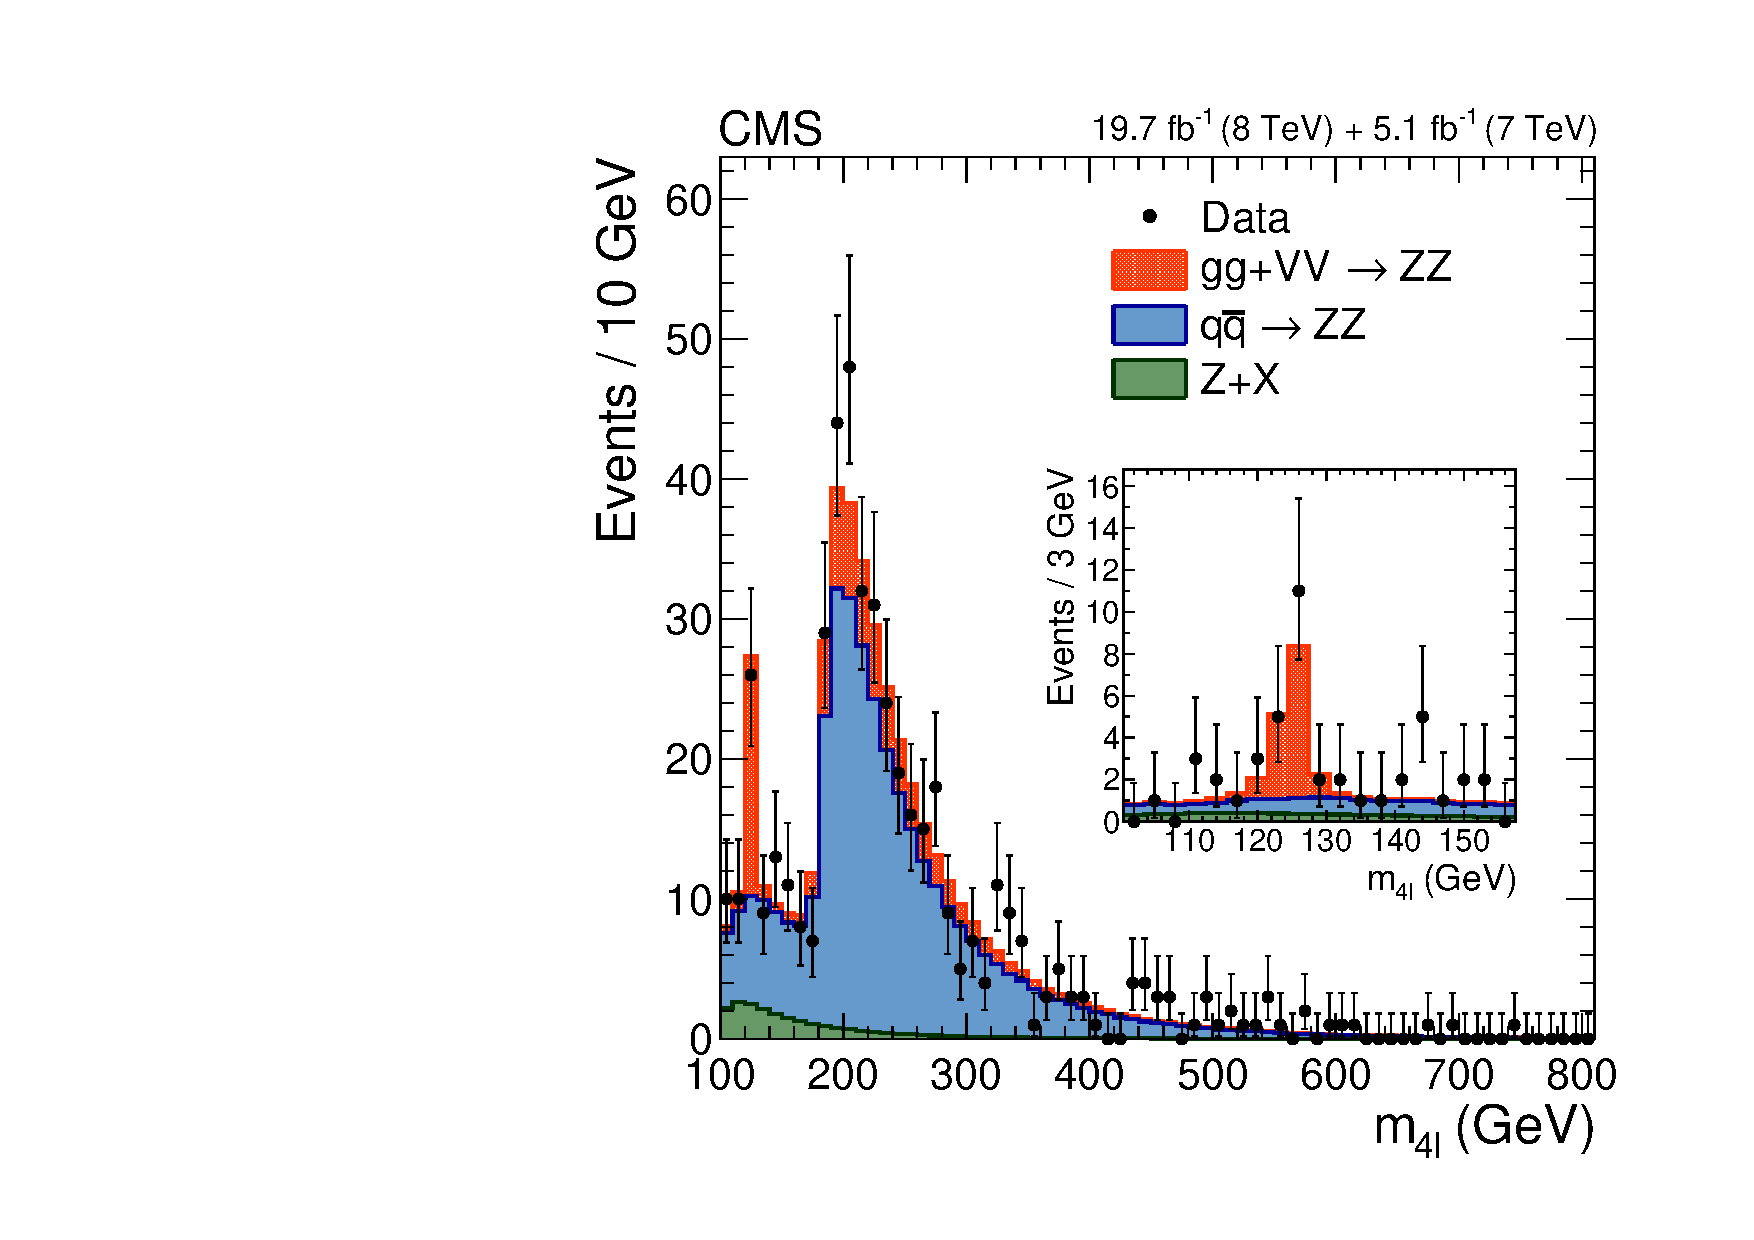
\includegraphics[width=\linewidth]{HZZ_Width/fig2_new.pdf}
\caption[Distribution of the four-lepton invariant mass in the range $100 < m_{4\ell} < \unit{800}{\GeV}$.
Points represent the data, filled histograms the expected contributions from the reducible
(Z+jets) and $q\bar{q}$ backgrounds, and from the sum of the gluon fusion (gg) and
vector boson fusion (VV) processes, including the Higgs boson mediated contributions.
The inset shows the distribution in the low mass region after a selection requirement
on the MELA likelihood discriminant $\mathcal{D}_\text{bkg}^\text{kin} > 0.5$.
In this region, the contribution of the $t\bar{t}H$ and VH production processes is added to
the dominant gluon fusion and VBF contributions.]{
Distribution of the four-lepton invariant mass in the range $100 < m_{4\ell} < \unit{800}{\GeV}$.
Points represent the data, filled histograms the expected contributions from the reducible
(Z+jets) and $q\bar{q}$ backgrounds, and from the sum of the gluon fusion (gg) and
vector boson fusion (VV) processes, including the Higgs boson mediated contributions.
The inset shows the distribution in the low mass region after a selection requirement
on the MELA likelihood discriminant $\mathcal{D}_\text{bkg}^\text{kin} > 0.5$~\cite{Chatrchyan:2013mxa}.
In this region, the contribution of the $t\bar{t}H$ and VH production processes is added to
the dominant gluon fusion and VBF contributions \cite{Khachatryan:2014iha}.
}
\label{fig:massfull}
\end{figure}

Focusing on the off mass resonance peak region, figure \ref{fig:mss-discr}(left) presents the $4\ell$ invariant mass distribution
for the off peak signal region ($m_{4\ell} > 220\GeV$) while the plot on the (right) presents the same region with an artificial cut on the MELA discriminant used in this analysis, $\mathcal{D}_{gg} > 0.65$, which will be introduced as the next kinematic distribution used in the analysis.
The expected contributions from the $q\bar{q} \to 4\ell$ and reducible backgrounds,
as well as for the total gluon fusion (gg) and vector boson fusion (VV) contributions, including the
Higgs boson signal, are shown. The expected m$_{4\ell}$ distributions for the sum of all the
processes, with a Higgs boson width $\Gamma_{H} = 10 \times \Gamma_{H}^{\mathrm{SM}}$ and a relative
cross section with respect to the SM cross section equal to unity in both gluon fusion and VBF production
modes, are also presented, showing the enhancement arising from the scaling of the squared product of the couplings. 

\begin{figure}
\centering
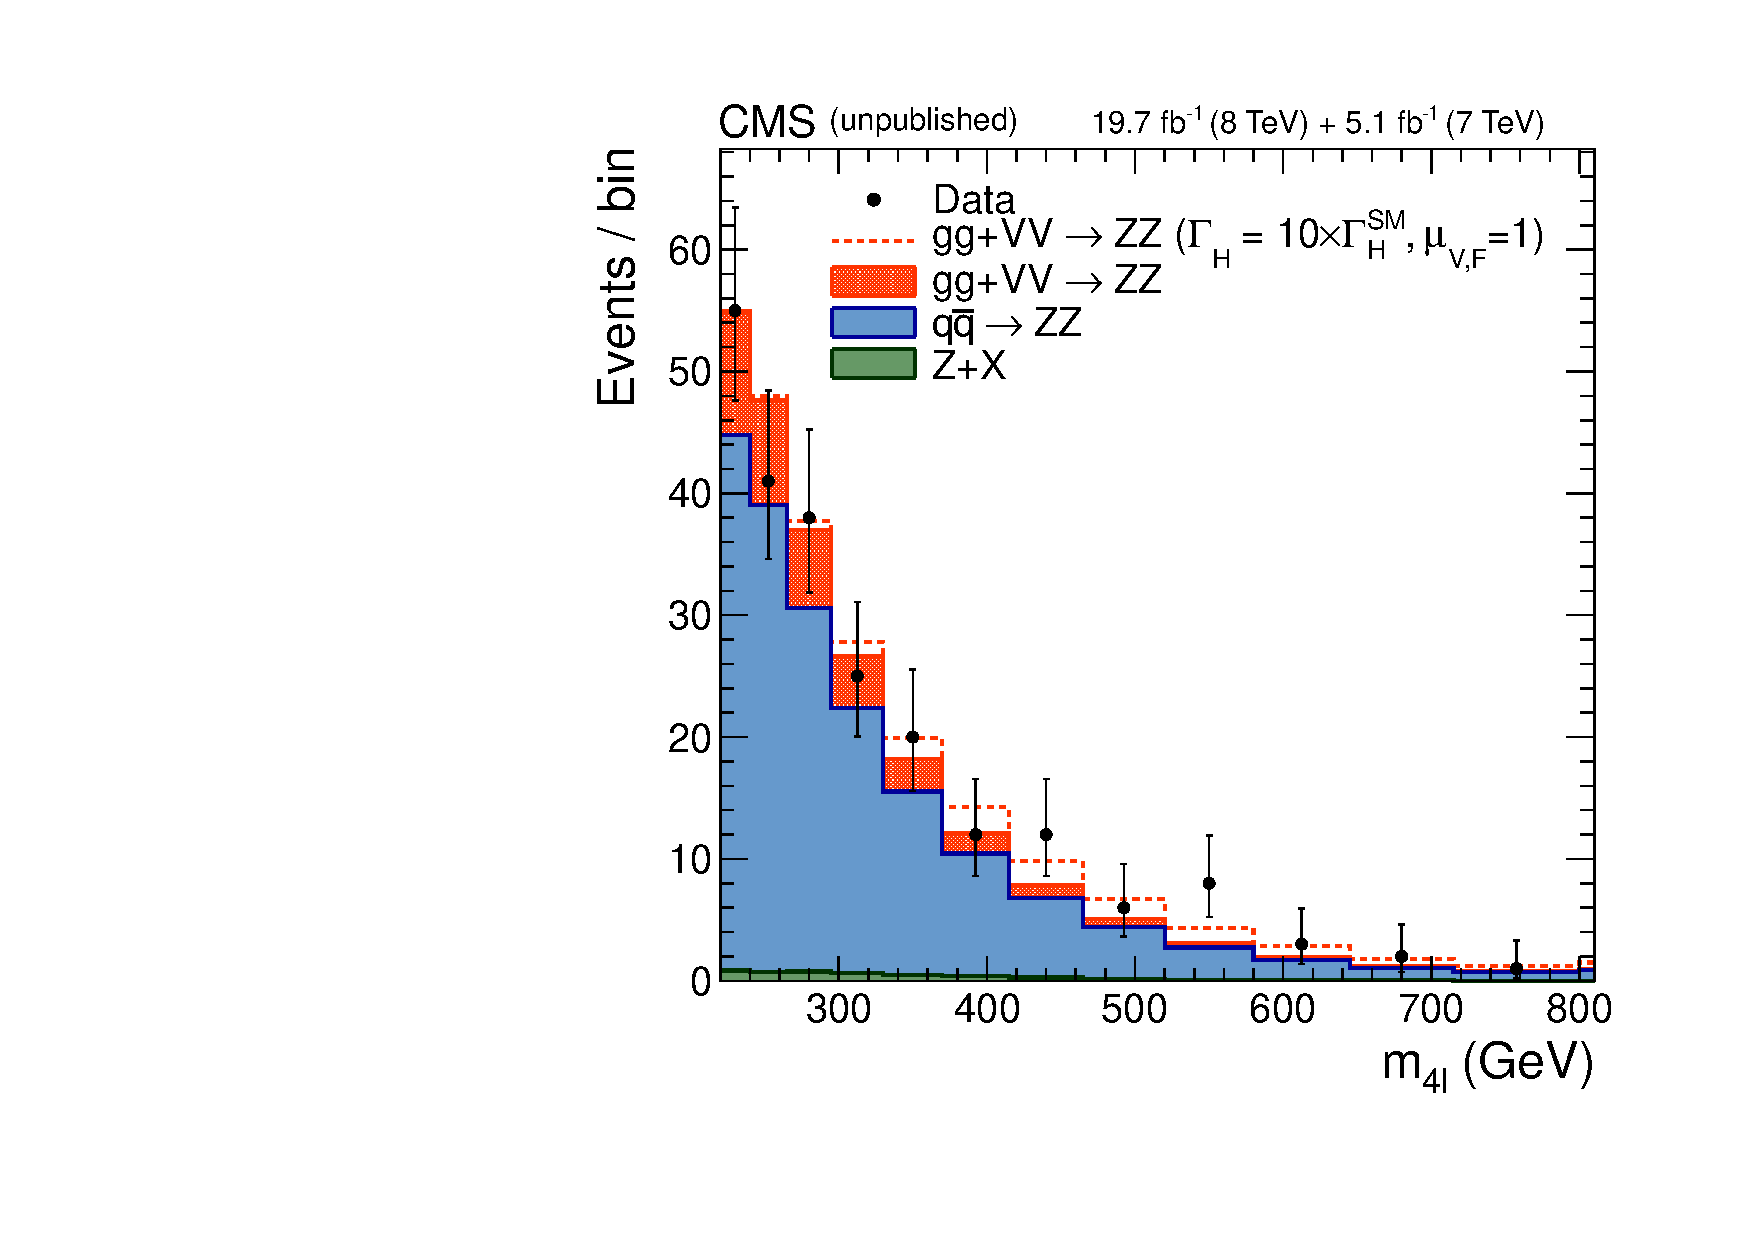
\includegraphics[width=0.475\textwidth]{HZZ_Width/ZZMass_AR_20May2014.pdf}
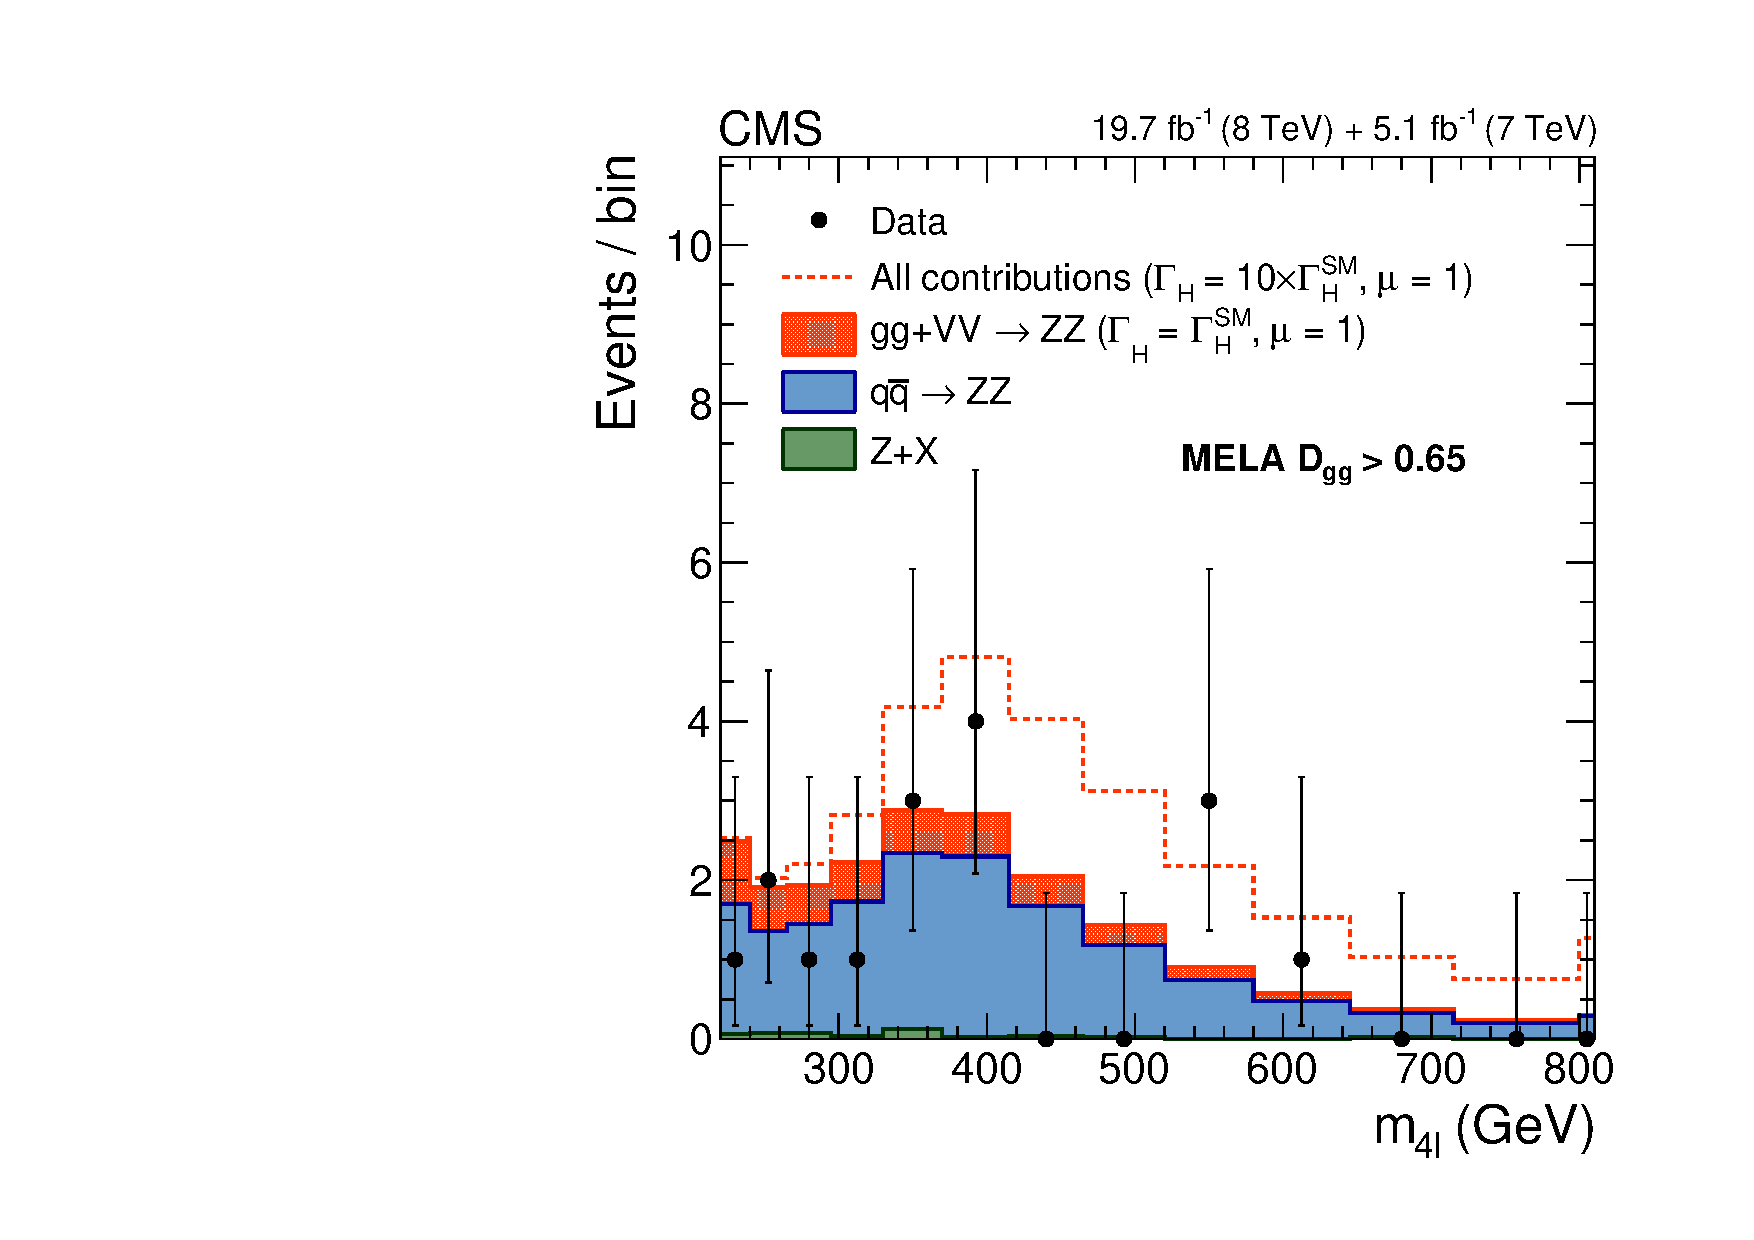
\includegraphics[width=0.45\textwidth]{HZZ_Width/fig3a_new.pdf}
\caption[Distributions of (left) the four-lepton invariant mass as used in that analysis (right) the four-lepton invariant mass after an artificial selection requirement
on the MELA likelihood discriminant $\mathcal{D}_{gg} > 0.65$. Points represent the data, filled histograms the expected
contributions from the reducible (Z+X) and $q\bar{q}$ backgrounds, and
from the gluon fusion (gg) and vector boson fusion (VV) SM processes (including
the Higgs boson mediated contributions). The dashed line corresponds to the total
expected yield for a Higgs boson width and a squared product of the couplings scaled by a
factor 10 with respect to their SM values.
In the top plot, the bin size varies from 20 to $\unit{85}{\GeV}$ and the last bin includes
all entries with masses above $\unit{800}{\GeV}$.]{
Distributions of (left) the four-lepton invariant mass as used in that analysis (right) the four-lepton invariant mass after an artificial selection requirement
on the MELA likelihood discriminant $\mathcal{D}_{gg} > 0.65$. Points represent the data, filled histograms the expected
contributions from the reducible (Z+X) and $q\bar{q}$ backgrounds, and
from the gluon fusion (gg) and vector boson fusion (VV) SM processes (including
the Higgs boson mediated contributions). The dashed line corresponds to the total
expected yield for a Higgs boson width and a squared product of the couplings scaled by a
factor 10 with respect to their SM values.
In the top plot, the bin size varies from 20 to $\unit{85}{\GeV}$ and the last bin includes
all entries with masses above $\unit{800}{\GeV}$ \cite{Khachatryan:2014iha}.
}
\label{fig:mss-discr}
\end{figure}

\subsection{$4\ell$ MELA discriminant}
\label{sec:MELA_gg}

In order to enhance the sensitivity to the gg production in the off peak region, a likelihood discriminant
$\mathcal{D}_{gg}$ is used, which characterizes the event topology in the $4\ell$ centre-of-mass frame
using the observables $(m_{Z_1}, m_{Z_2}, \vec\Omega)$ for a given value of $m_{4\ell}$, where
$\vec\Omega$ denotes the five angles defined in the previous sections. The discriminant is built from the
probabilities $\mathcal{P}^{gg}_\text{tot}$ and $\mathcal{P}^{q\bar{q}}_\text{bkg}$
for an event to originate from either the $gg \to 4\ell$ or the $q\bar{q} \to 4\ell$
process. We use the matrix element likelihood approach (MELA)~\cite{Chatrchyan:2012ufa, Bolognesi:2012mm}
for the probability computation using the \textsc{MCFM} matrix elements for both $gg \to 4\ell$ and
$q\bar{q} \to 4\ell$ processes.
The probability $\mathcal{P}^{gg}_\text{tot}$ for the $gg \to 4\ell$ process includes
the signal ($\mathcal{P}^{gg}_\text{sig}$), the background ($\mathcal{P}^{gg}_\text{bkg}$),
and their interference ($\mathcal{P}^{gg}_\text{int}$), as introduced for the discriminant computation~\cite{Anderson:2013afp}. The discriminant is defined as
\begin{equation}
\label{eq:kd-ggmela}
\mathcal{D}_{gg} = \frac{\mathcal{P}^{gg}_\text{tot}  }{\mathcal{P}^{gg}_\text{tot}  + \mathcal{P}^{q\bar{q}}_\text{bkg} }=
\left[1+\frac{\mathcal{P}^{q\bar{q}}_\text{bkg}  }
{a \times \mathcal{P}^{gg}_\text{sig} +  \sqrt{a} \times  \mathcal{P}^{gg}_\text{int} + \mathcal{P}^{gg}_\text{bkg}  } \right]^{-1} ,
\end{equation}
where
the parameter $a$ is the strength of the unknown anomalous $gg$ contribution with respect to the
expected SM contribution ($a=1$). We set $a = 10$ in the definition of $\mathcal{D}_{gg}$ according
to the expected sensitivity. Studies show that the expected sensitivity of the analysis is relatively independent of the value of $a$ chosen\footnote{Values within a factor of 2.}. It should be stressed that fixing the parameter $a$ to
a given value only affects the sensitivity of the analysis. 

Individual distributions of the kinematic variables input into the $\mathcal{D}_{gg}$ calculation are shown in figure \ref{fig:Width_KD_inputs} for a gg enriched selection of $m_{4\ell} > \unit{330}{\GeV}$. These are simplified by summing together the $m_{Z_{1}}$ and $m_{Z_{2}}$ and $\cos\theta_{1}$ and $\cos\theta_{2}$ distributions.

\begin{figure}
\centering
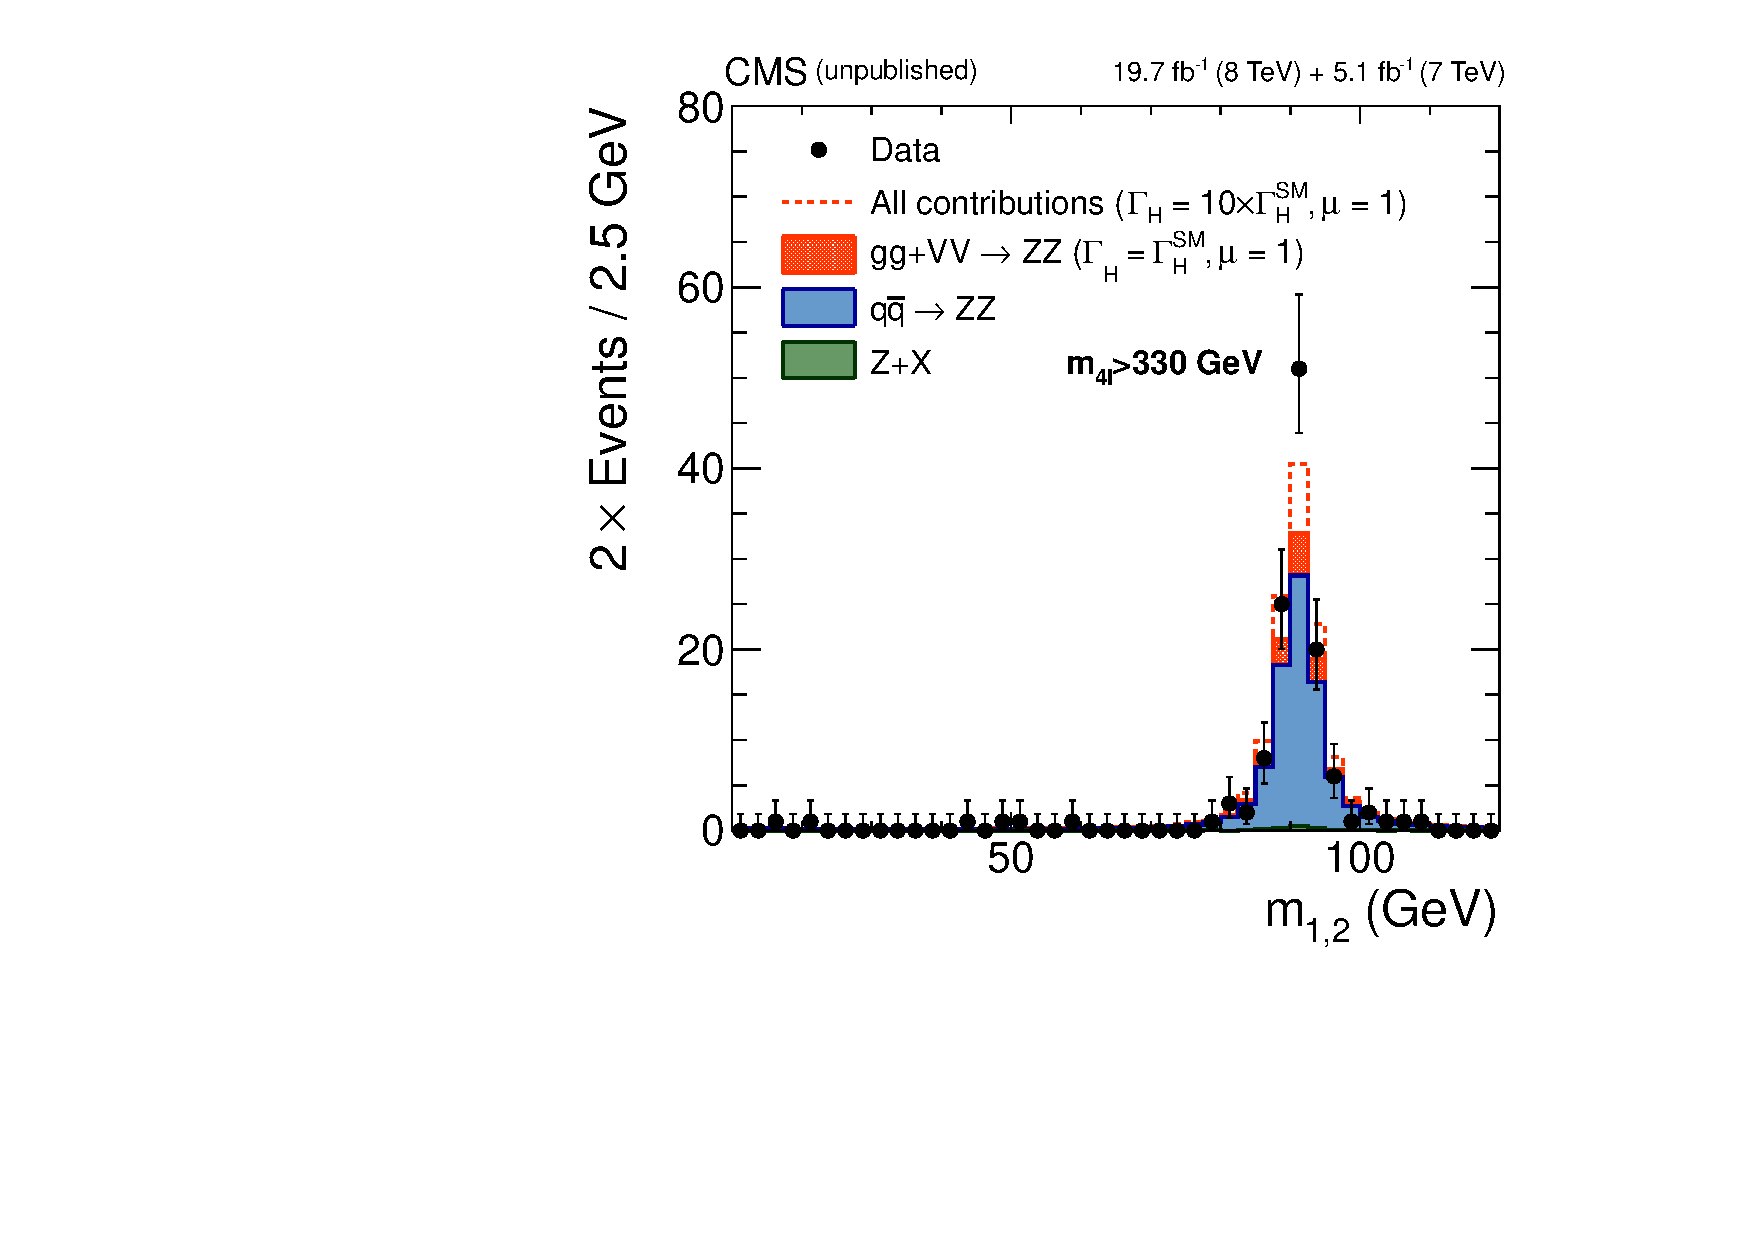
\includegraphics[width=0.32\textwidth]{HZZ_Width/cCompare_DataMC_AllTeV_avgMZ_330.pdf}
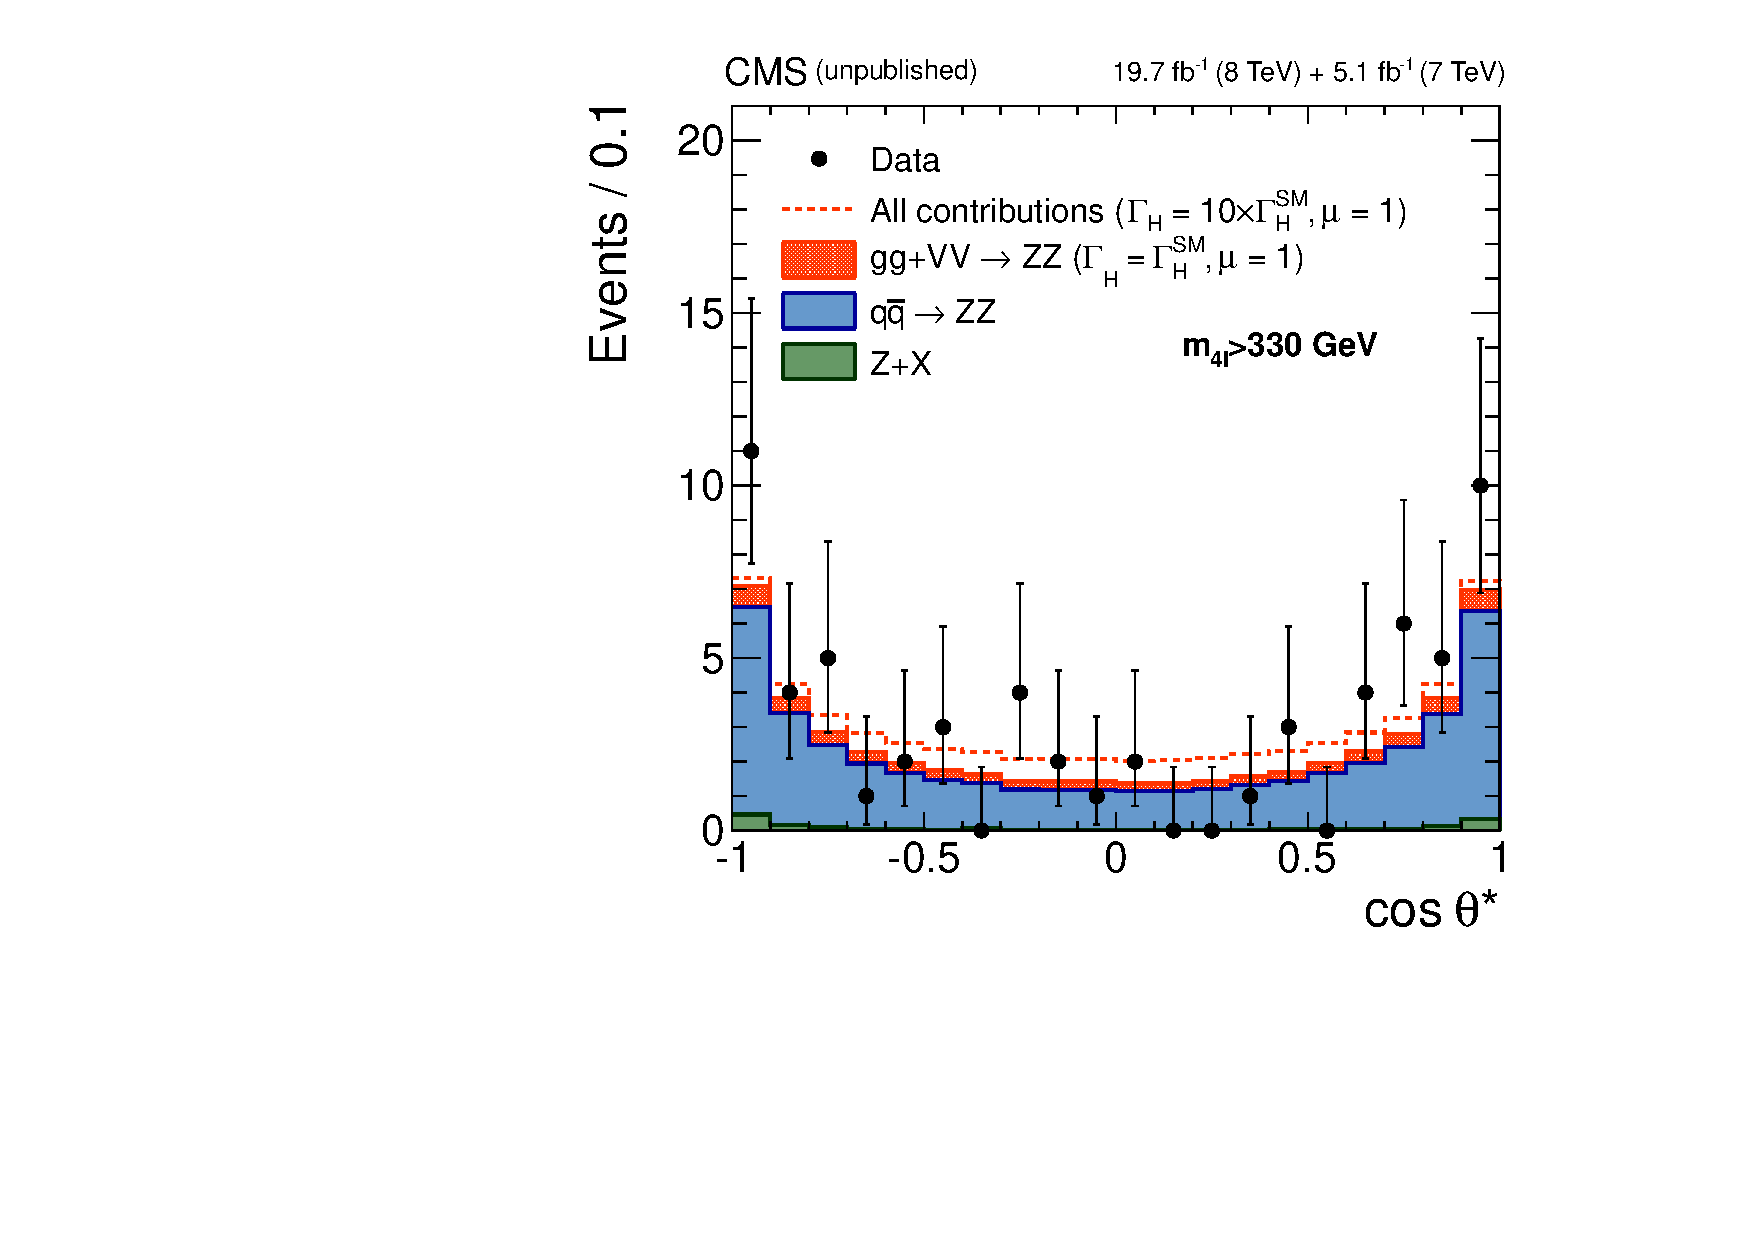
\includegraphics[width=0.32\textwidth]{HZZ_Width/cCompare_DataMC_AllTeV_ZS_330.pdf} 
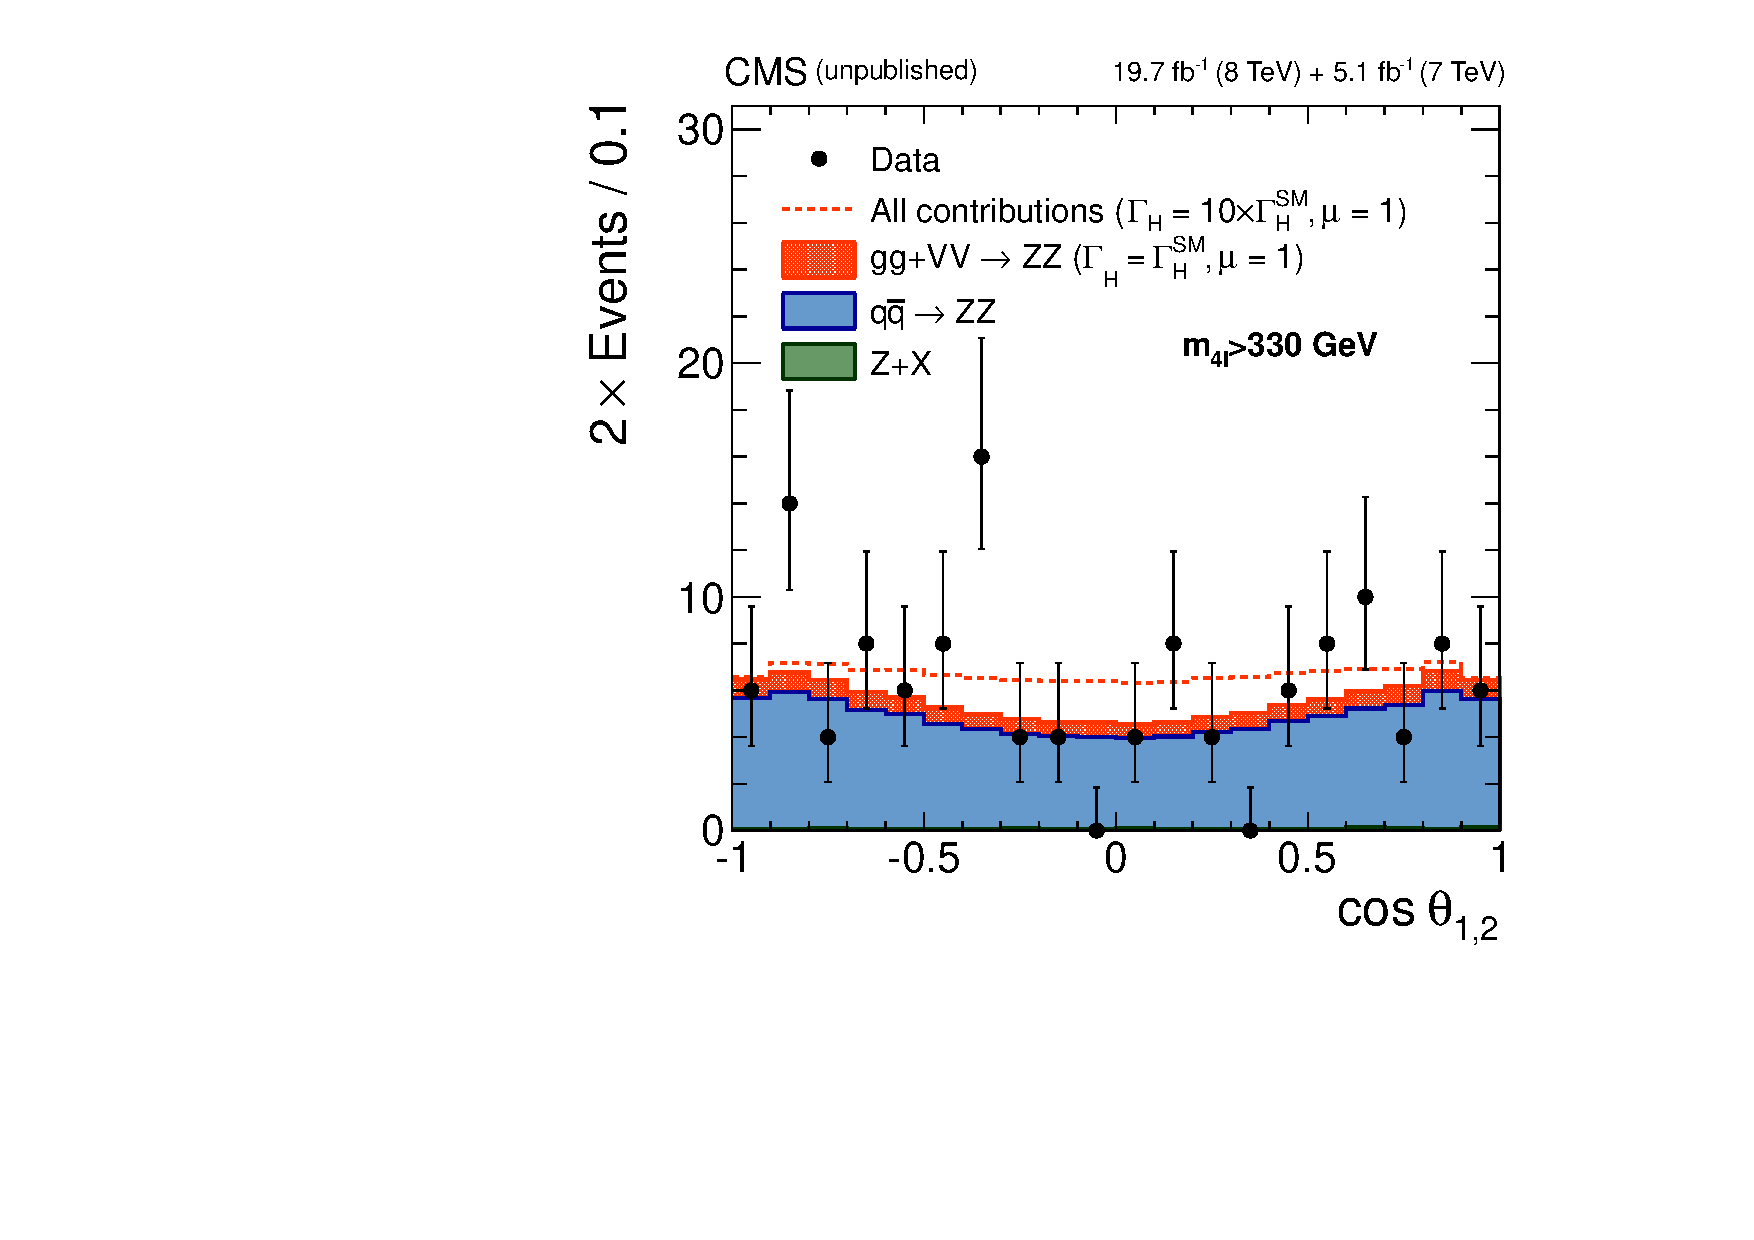
\includegraphics[width=0.32\textwidth]{HZZ_Width/cCompare_DataMC_AllTeV_h1h2_330.pdf} \\
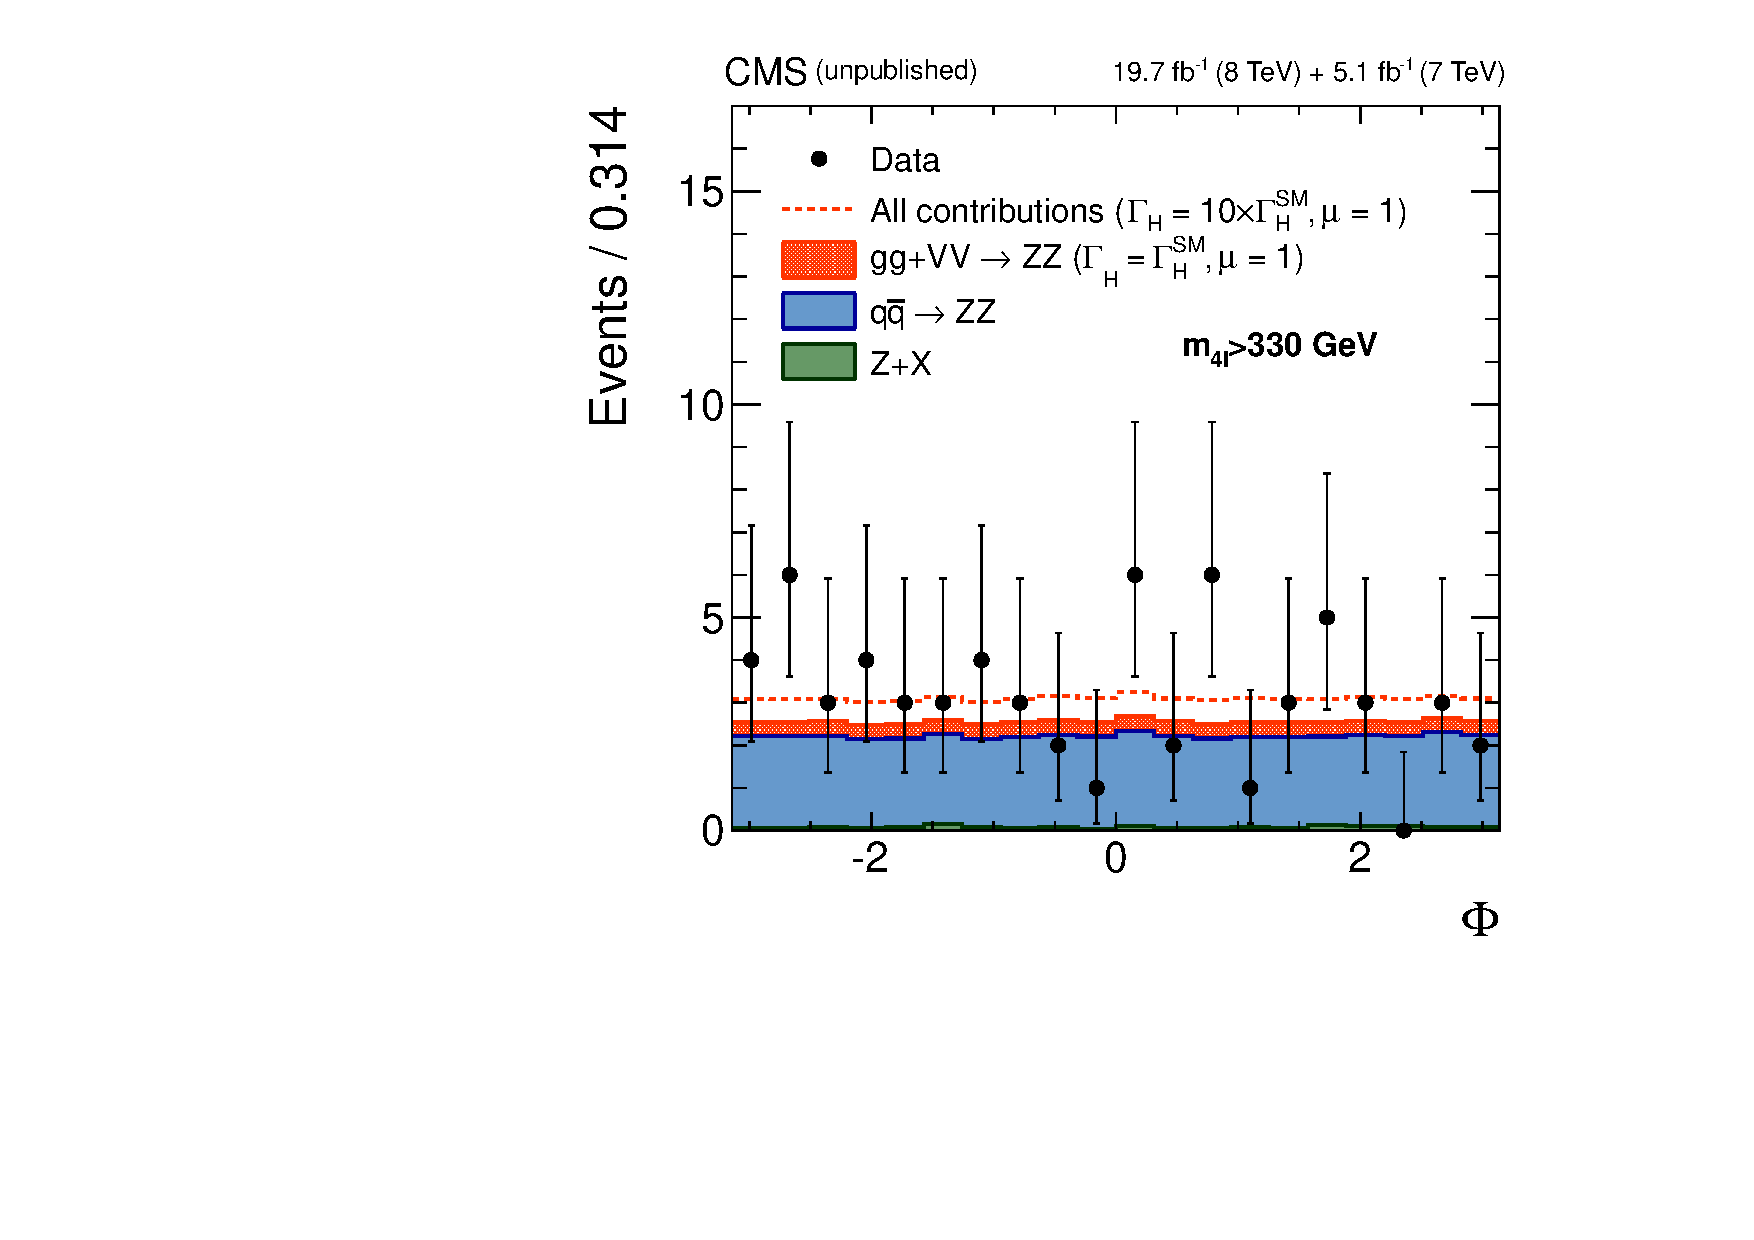
\includegraphics[width=0.32\textwidth]{HZZ_Width/cCompare_DataMC_AllTeV_helphi_330.pdf}
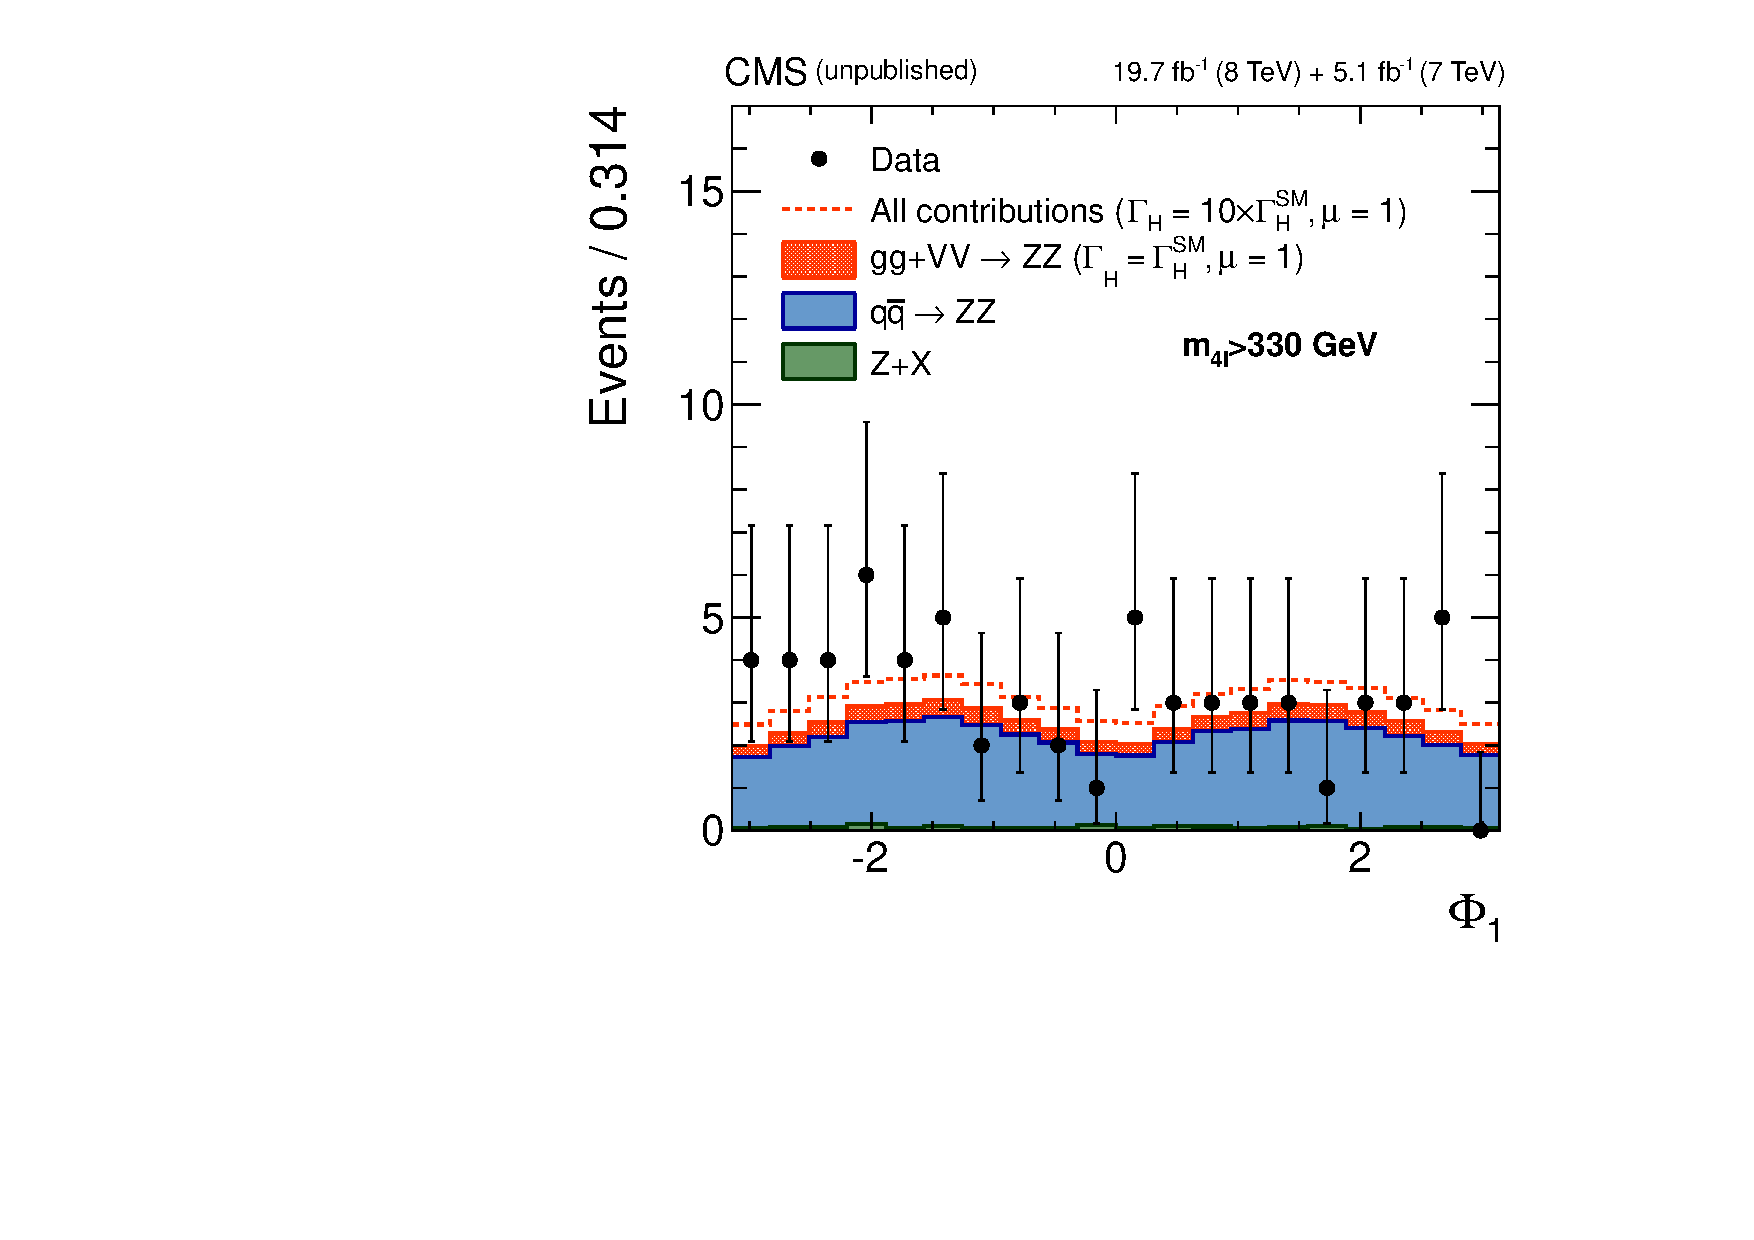
\includegraphics[width=0.32\textwidth]{HZZ_Width/cCompare_DataMC_AllTeV_phi_330.pdf}
\caption[Distributions of the kinematic observables used in the $\mathcal{D}_{gg}$ discriminant:
$m_{Z_i}$, $\cos\theta^*$, $\cos\theta_{i}$, $\Phi$, and $\Phi_{1}$. The distributions for $m_{Z_{1}}$ and $m_{Z_{2}}$ and $\cos\theta_{1}$ and $\cos\theta_{2}$ are summed together. The observed data (points with error bars), the expectations for the SM background (shaded areas),
the SM Higgs boson signal (open areas under the solid histogram), and the Higgs boson width $\Gamma_{H} = 10 \times \Gamma_{H}^{\mathrm{SM}}$ are shown. The mass of the resonance is taken to be $\unit{125.6}{\GeV}$ and the gg enriched off resonance region is shown $m_{4\ell} > \unit{330}{\GeV}$.]{ Distributions of the eight kinematic observables used in the $\mathcal{D}_{gg}$ discriminant:
$m_{Z_i}$, $\cos\theta^*$, $\cos\theta_{i}$, $\Phi$, and $\Phi_{1}$. The distributions for $m_{Z_{1}}$ and $m_{Z_{2}}$ and $\cos\theta_{1}$ and $\cos\theta_{2}$ are summed together. The observed data (points with error bars), the expectations for the SM background (shaded areas),
the SM Higgs boson signal (open areas under the solid histogram), and the Higgs boson width $\Gamma_{H} = 10 \times \Gamma_{H}^{\mathrm{SM}}$ are shown. The mass of the resonance is taken to be $\unit{125.6}{\GeV}$ and the gg enriched off resonance region is shown $m_{4\ell} > \unit{330}{\GeV}$\cite{Khachatryan:2014iha}.}
\label{fig:Width_KD_inputs}
\end{figure}

Figure \ref{fig:kd-discr}(left) presents the $\mathcal{D}_{gg}$ invariant mass distribution
for the off peak signal region ($m_{4\ell} > 220\GeV$) while the plot on the (right) presents the same region with an artificial cut on the mass, $m_{4\ell} > \unit{330}{\GeV}$.
The expected contributions from the $q\bar{q} \to 4\ell$ and reducible backgrounds,
as well as for the total gluon fusion (gg) and vector boson fusion (VV) contributions, including the
Higgs boson signal, are shown. The expected kinematic distributions for the sum of all the
processes, with a Higgs boson width $\Gamma_{H} = 10 \times \Gamma_{H}^{\mathrm{SM}}$ and a relative
cross section with respect to the SM cross section equal to unity in both gluon fusion and VBF production
modes, are also presented, showing the enhancement arising from the scaling of the squared product of the couplings. 

\begin{figure}
\centering
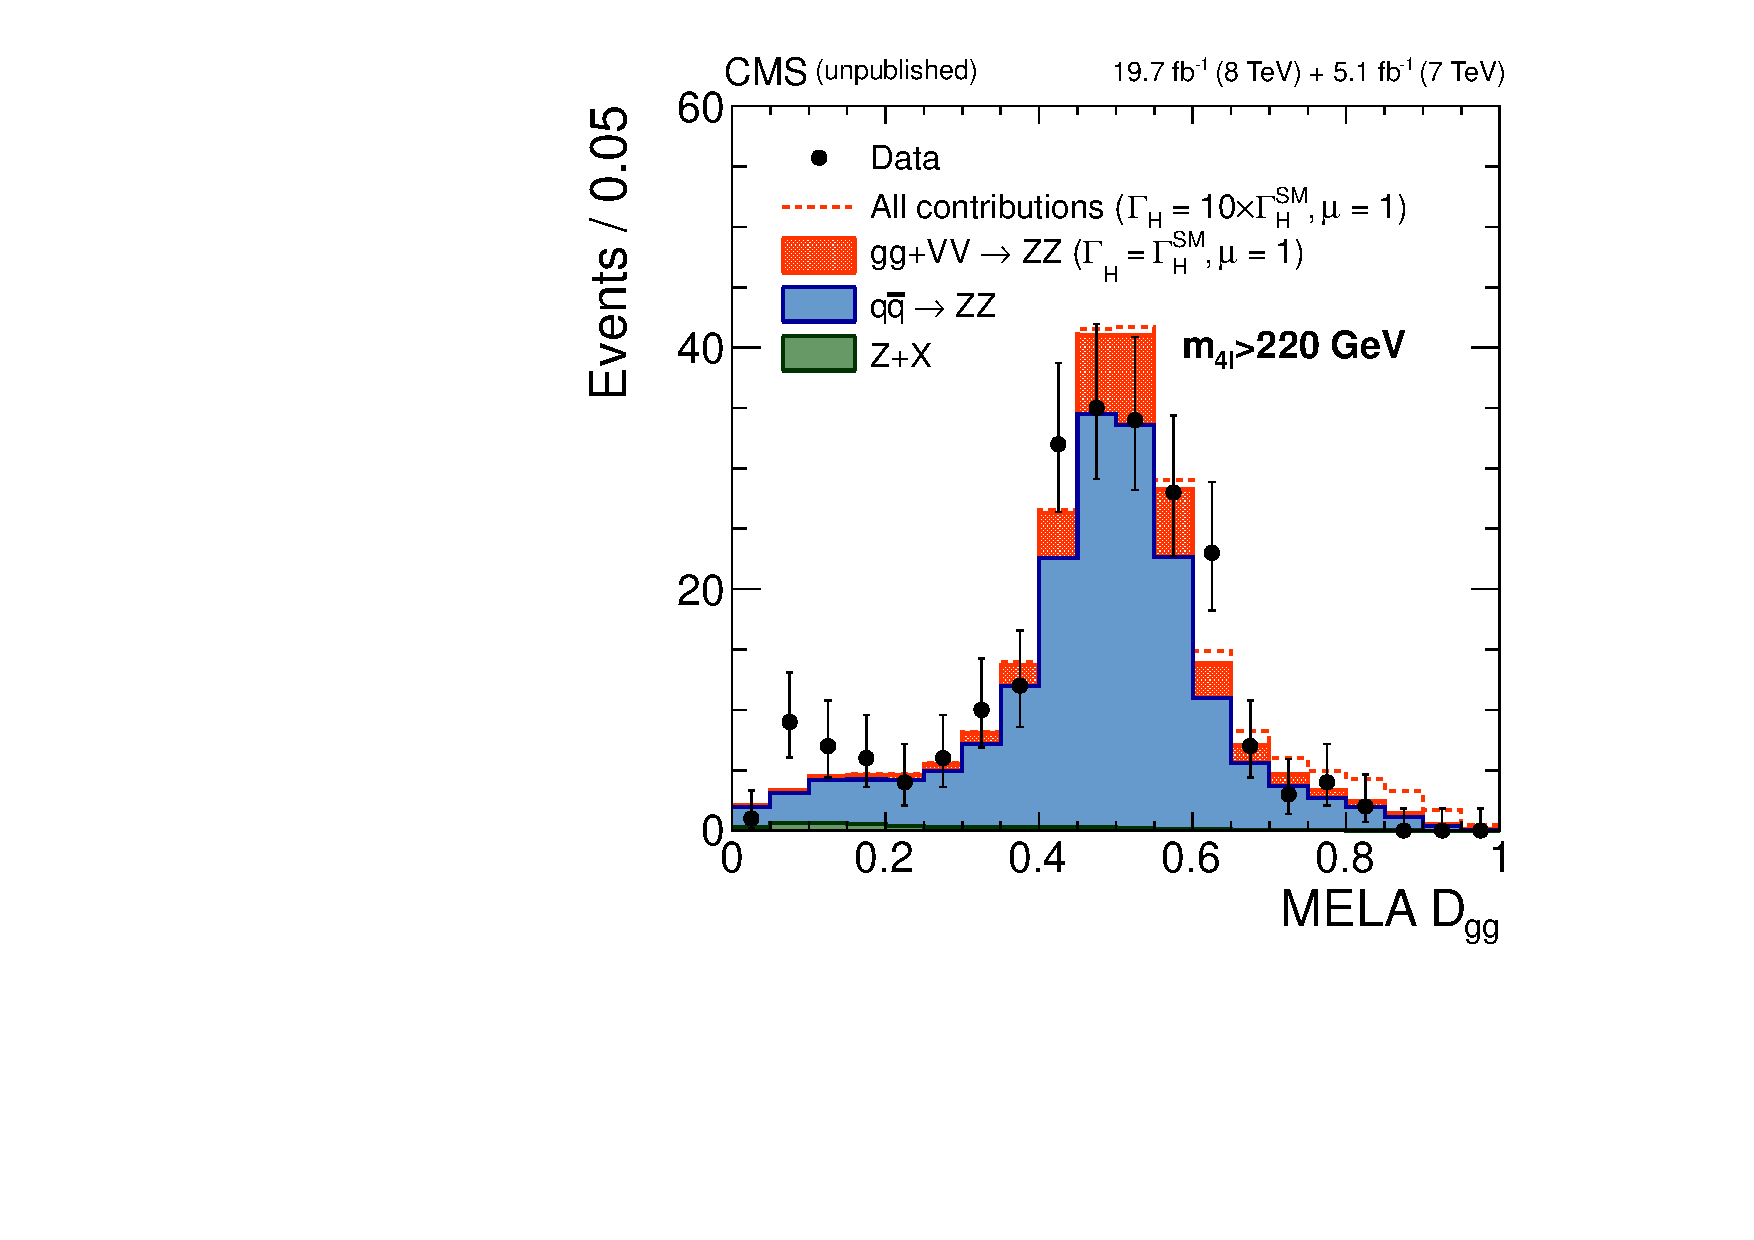
\includegraphics[width=0.475\textwidth]{HZZ_Width/cCompare_DataMC_AllTeV_Dgg10__Low220.pdf}
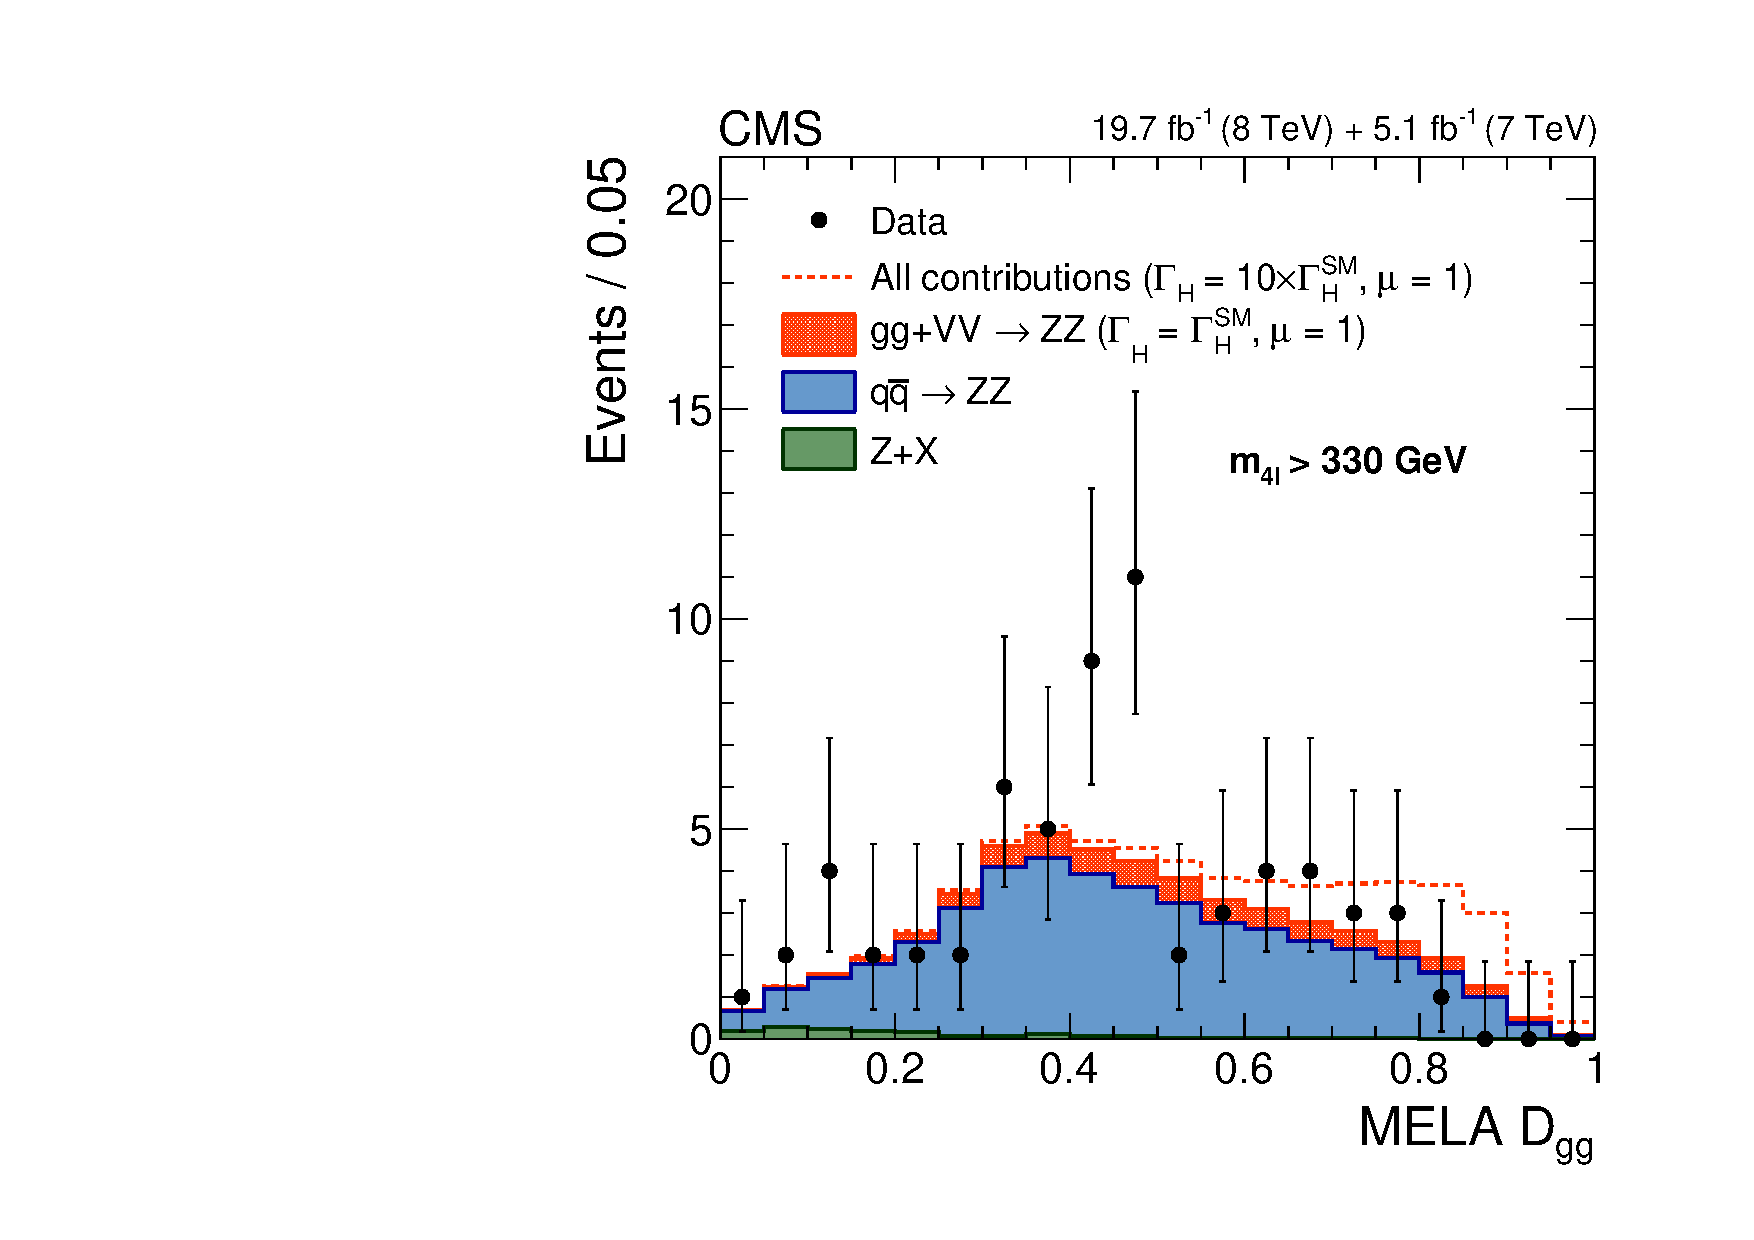
\includegraphics[width=0.45\textwidth]{HZZ_Width/fig3b_new.pdf}
\caption[(left) Distribution of the MELA discriminant $\mathcal{D}_{gg}$ in full analysis mass range for the sum of the $4e$, $4\mu$, and $2e2\mu$ channels. Points represent the data, shaded histograms represent the background and dotted-shaded histogram the $gg+VV \to ZZ$ expectations for a Higgs mass of $\unit{125.6}{\GeV}$. The expected distributions are presented as stacked histograms. The measurements are presented for of the data collected at $\sqrt{s} = 7$ and $\unit{8}{\TeV}$ in the $\unit{220--1600}{\GeV}$ range. (right) The $\mathcal{D}_{gg}$ likelihood discriminant for $m_{4\ell} > \unit{330}{\GeV}$ in the $4\ell$ channel. Points represent the data, filled histograms the expected contributions from the reducible (Z+jets) and $q\bar{q}$ backgrounds, and from the gluon fusion (gg) and vector boson fusion (VV) SM processes (including the Higgs boson mediated contributions). The dashed line corresponds to the total expected yield for a Higgs boson width and a squared product of the couplings scaled by a factor 10 with respect to their SM values.]
{
(left) Distribution of the MELA discriminant $\mathcal{D}_{gg}$ in full analysis mass range for the sum of the $4e$, $4\mu$, and $2e2\mu$ channels. Points represent the data, shaded histograms represent the background and dotted-shaded histogram the $gg+VV \to ZZ$ expectations for a Higgs mass of $\unit{125.6}{\GeV}$. The expected distributions are presented as stacked histograms. The measurements are presented for of the data collected at $\sqrt{s} = 7$ and $\unit{8}{\TeV}$ in the $\unit{220--1600}{\GeV}$ range. (right) The $\mathcal{D}_{gg}$ likelihood discriminant for $m_{4\ell} > \unit{330}{\GeV}$ in the $4\ell$ channel. Points represent the data, filled histograms the expected contributions from the reducible (Z+jets) and $q\bar{q}$ backgrounds, and from the gluon fusion (gg) and vector boson fusion (VV) SM processes (including the Higgs boson mediated contributions). The dashed line corresponds to the total expected yield for a Higgs boson width and a squared product of the couplings scaled by a factor 10 with respect to their SM values \cite{Khachatryan:2014iha}.
}
\label{fig:kd-discr}
\end{figure}

\subsection{$2\ell2\nu$ $m_{T}$ discriminant}
\label{sec:2l2nu_mT}

The previous section introduced the $m_{T}$ variable and that is an important distribution used to define the $2\ell2\nu$ signal region. It is also used as a kinematic distribution used in the final likelihood fit. Shown in figure \ref{fig:mtfit}, the off resonance $m_{T}$ distribution contains information about the width of the boson observed in the $4\ell$ final state. This distribution is used as a one-dimensional shape discriminant in each of the categories in this final state.


\begin{figure}[htb]
\centering
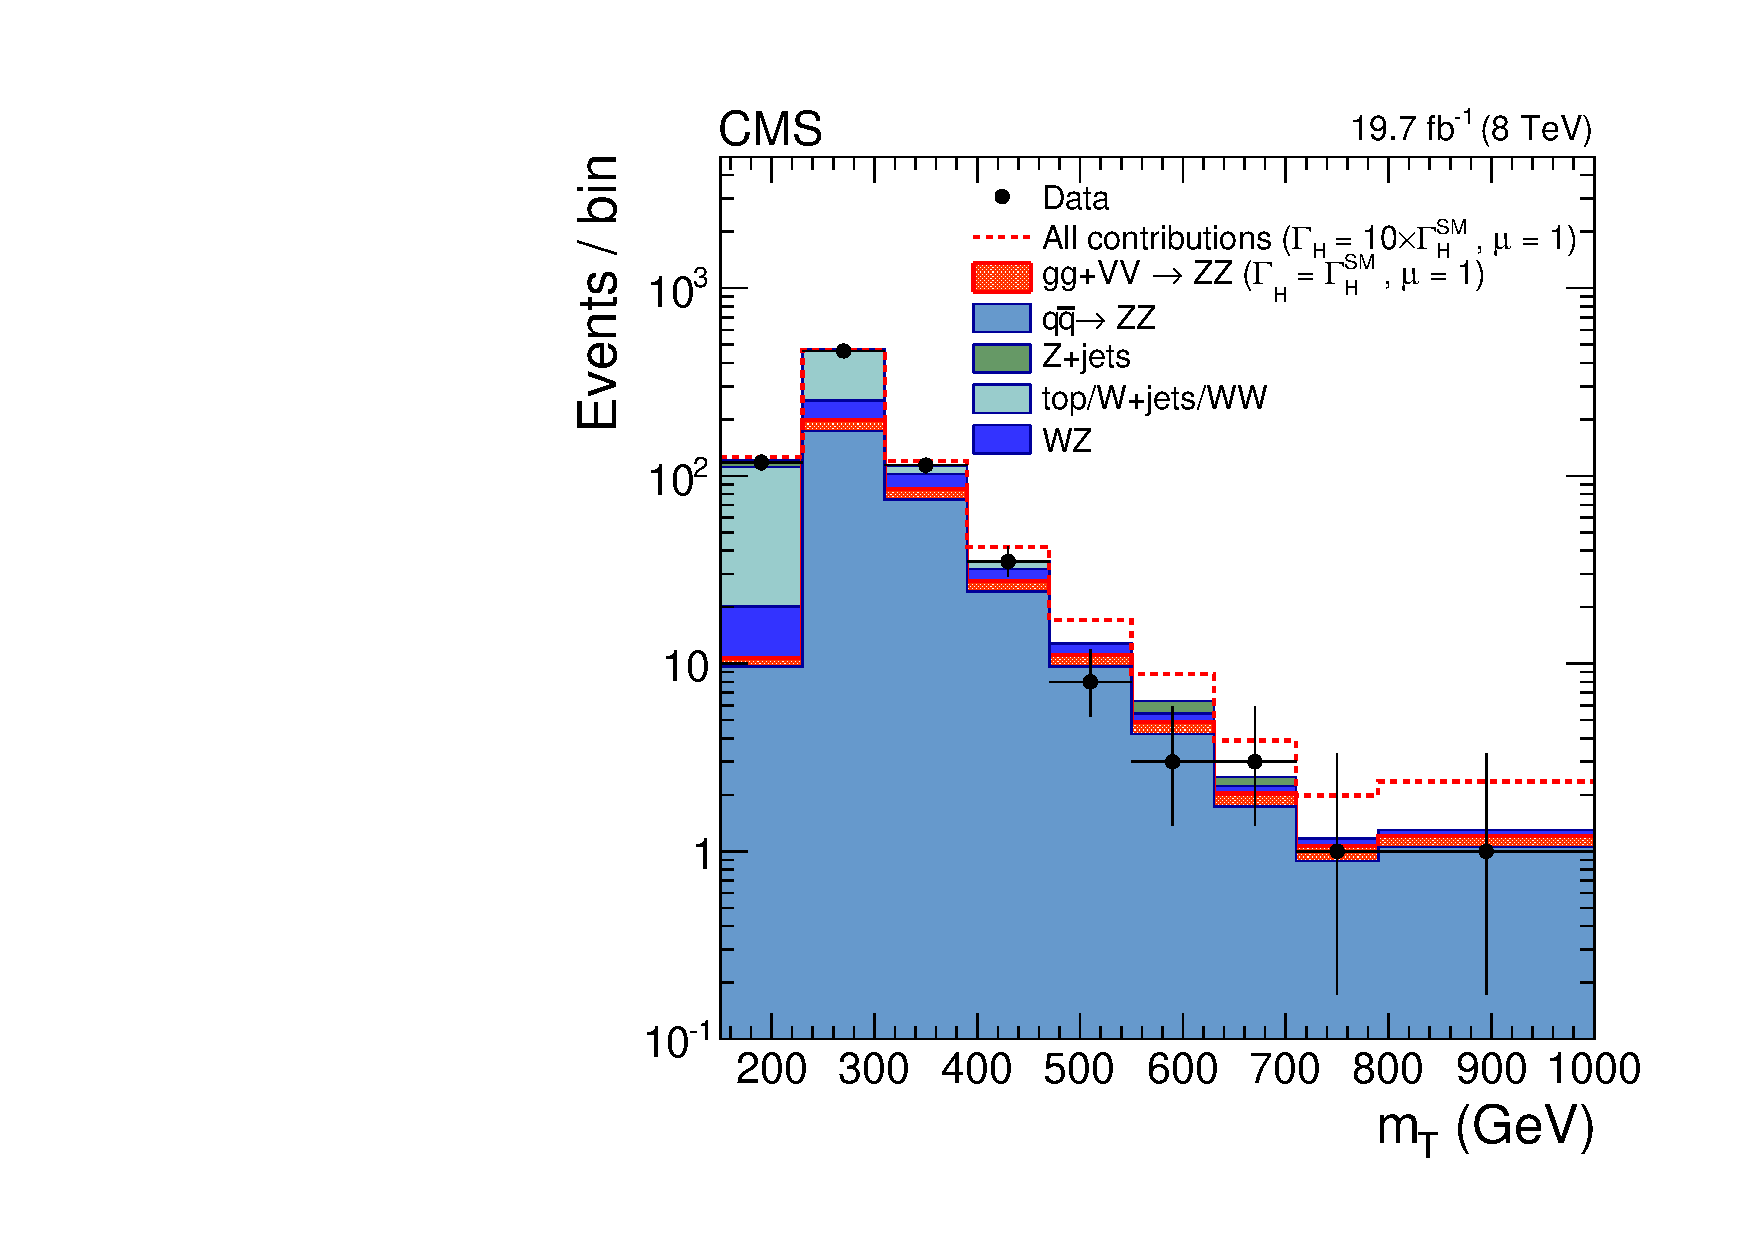
\includegraphics[width=0.45\linewidth]{HZZ_Width/fig4_new.pdf}
\caption[Distribution of the transverse mass in the $2\ell2\nu$ channel. Points represent
the data, filled histograms the expected contributions from the backgrounds, and
from the gluon fusion (gg) and vector boson fusion (VV) SM processes (including
the Higgs-mediated contributions). The dashed line corresponds to the total expected
yield for a Higgs boson width and a squared product of the couplings scaled by a
factor 10 with respect to their SM values.
The bin size varies from 80 to $\unit{210}{\GeV}$ and the last bin includes all entries with
transverse masses above $\unit{1}{\TeV}$.]{
Distribution of the transverse mass in the $2\ell2\nu$ channel. Points represent
the data, filled histograms the expected contributions from the backgrounds, and
from the gluon fusion (gg) and vector boson fusion (VV) SM processes (including
the Higgs-mediated contributions). The dashed line corresponds to the total expected
yield for a Higgs boson width and a squared product of the couplings scaled by a
factor 10 with respect to their SM values.
The bin size varies from 80 to $\unit{210}{\GeV}$ and the last bin includes all entries with
transverse masses above $\unit{1}{\TeV}$ \cite{Khachatryan:2014iha}.}
\label{fig:mtfit}
\end{figure}


\section{Off Resonance Width Results}
\label{sec:Width_Results}

In the $4\ell$ final state the number of observed events for the high mass region ($m_{4l} \ge \unit{220}{\GeV}$) as well as the number of expected events for the signal, the background and the interference contributions are presented on table~\ref{tab:4l_width_yields}. A good agreement is observed between the measured and total expected yields. Yields for the low-mass region ($105.6 \ge m_{4l} \ge \unit{140.6}{\GeV}$) are taken from the previous section~\cite{Chatrchyan:2013mxa}. As an illustration of the sensitivity of the kinematic variables used in this analysis, a modified set of yields are presented where the selection is modified from the actual analysis to the gg enhanced region, table \ref{tab:yields}

\begin{table}
\begin{center}
\begin{tabular}{l|c|c|c|c}
 \hline
\hline
Final state & $4e$  &  $2e2\mu$  & $4\mu$  & $4\ell$ \\
\hline
gg signal (SM) &  0.50 $^{+0.07}_{-0.06}$ & 1.19 $^{+0.13}_{-0.14}$ &  0.70 $^{+0.09}_{-0.09}$ &  2.39 $^{+0.17}_{-0.19}$  \\
gg background &  7.5 $^{+1.4}_{-1.1}$  & 17.9 $^{+2.8}_{-3.0}$  & 10.8 $^{+1.6}_{-1.6}$ &  36.2 $^{+3.4}_{-3.6}$  \\
total gg (SM) & 7.1  $^{+1.2}_{-1.2}$ & 17.0 $^{+2.5}_{-2.6}$ & 9.9  $^{+1.4}_{-1.6}$ & 34.0 $^{+3.0}_{-3.1}$  \\
\hline
VBF signal (SM) & 0.048 & 0.115 & 0.065 & 0.228  \\                                                                       
VBF background & 0.49 & 1.17 & 0.67 & 2.33  \\                                                                             
total VBF (SM) & 0.43 & 1.03 & 0.59 & 2.05  \\
\hline
$q\bar{q}$ & 36.2 $\pm 4.0$  & 87.9 $\pm 6.4$  & 53.0 $\pm 3.6$  & 177.1 $\pm 8.1$   \\
reducible & 2.2 $\pm 0.5$ & 1.7 $\pm 0.4$ & 0.6 $\pm 0.2$ & 4.5 $\pm 0.7$  \\
\hline
All contributions (SM) & 45.9 $\pm 4.3$  & 107.6 $\pm 7.1$ & 64.1 $^{+3.9}_{-4.0}$  & 217.6 $\pm 9.5$ \\
\hline
Observed  & 41 & 122 & 60 & 223 \\
\hline
\end{tabular}
\caption[Expected and observed number of events for $m_{ZZ} \ge \unit{220}{\GeV}$ per channel and for the sum of the
$4e$, $4\mu$ and $2e2\mu$ channels. The numbers for the gg signal and the total gg contribution are given for $\mu=1$ (SM). 
The numbers correspond to the sum of 7 and $\unit{8}{\TeV}$ data. VBF errors are negligible with respect to the corresponding gg sources, 
so they are not reported.]{Expected and observed number of events for $m_{ZZ} \ge \unit{220}{\GeV}$ per channel and for the sum of the
$4e$, $4\mu$ and $2e2\mu$ channels. The numbers for the gg signal and the total gg contribution are given for $\mu=1$ (SM). 
The numbers correspond to the sum of 7 and $\unit{8}{\TeV}$ data. VBF errors are negligible with respect to the corresponding gg sources, 
so they are not reported \cite{Khachatryan:2014iha}.} 
\label{tab:4l_width_yields}
\end{center}
\end{table}

\begin{table}
\centering
\caption[Expected and observed numbers of events in the $4\ell$ and $2\ell2\nu$
channels in $gg$-enriched regions, defined by $m_{4\ell} \ge \unit{330}{\GeV}$ and
$\mathcal{D}_{gg} >$ 0.65 ($4\ell$), and by $m_{T} >\unit{350}{\GeV}$ and $E_{T}^{\text{miss}} > \unit{100}{\GeV}$ ($2\ell2\nu$).
The numbers of expected events are given separately for the gg and VBF processes,
and for a SM Higgs boson ($\Gamma_{H} = \Gamma_{H}^{\mathrm{SM}}$) and a Higgs
boson width and squared product of the couplings scaled by a
factor 10 with respect to their SM values. The unphysical
expected contributions for the signal and background components are also reported
separately, for the gg and VBF processes. For both processes, the sum of the signal
and background components differs from the total due to the negative interferences.
The quoted uncertainties include only the systematic sources.]{Expected and observed numbers of events in the $4\ell$ and $2\ell2\nu$
channels in $gg$-enriched regions, defined by $m_{4\ell} \ge \unit{330}{\GeV}$ and
$\mathcal{D}_{gg} >$ 0.65 ($4\ell$), and by $m_{T} >\unit{350}{\GeV}$ and $E_{T}^{\text{miss}} > \unit{100}{\GeV}$ ($2\ell2\nu$).
The numbers of expected events are given separately for the gg and VBF processes,
and for a SM Higgs boson ($\Gamma_{H} = \Gamma_{H}^{\mathrm{SM}}$) and a Higgs
boson width and squared product of the couplings scaled by a
factor 10 with respect to their SM values. The unphysical
expected contributions for the signal and background components are also reported
separately, for the gg and VBF processes. For both processes, the sum of the signal
and background components differs from the total due to the negative interferences.
The quoted uncertainties include only the systematic sources \cite{Khachatryan:2014iha}.
}
\begin{tabular}{clccc}
\hline
\hline
 &                                       &  $4\ell$ & $2\ell 2\nu$ \\
\hline
(a)& Total $gg$ ($\Gamma_{H }= \Gamma_{H}^{\mathrm{SM}}$)  & 1.8\,$\pm 0.3$  & 9.6\,$\pm 1.5$ & \\
 & $gg$ Signal component ($\Gamma_{H} = \Gamma_{H}^{\mathrm{SM}}$)   & 1.3\,$\pm 0.2$  & 4.7\,$\pm 0.6$ & \\
 & $gg$ Background component                                          & 2.3\,$\pm 0.4$  & 10.8\,$\pm 1.7$  & \\
(b)& Total $gg$ ($\Gamma_{H} = 10 \times \Gamma_{H}^{\mathrm{SM}}$) & 9.9\,$\pm 1.2$  & 39.8\,$\pm5.2$ & \\
\hline
(c)& Total VBF ($\Gamma_{H} = \Gamma_{H}^{\mathrm{SM}}$)         & 0.23\,$\pm 0.01$    & 0.90\,$\pm 0.05$ & \\
 & VBF signal component ($\Gamma_{H} = \Gamma_{H}^{\mathrm{SM}}$)          & 0.11\,$\pm 0.01$    & 0.32\,$\pm 0.02$ & \\
 & VBF background component                                                  & 0.35$\pm 0.02$      & 1.22\,$\pm 0.07$ & \\
(d)& Total VBF ($\Gamma_{H} = 10 \times \Gamma_{H}^{\mathrm{SM}}$)        & 0.77\,$\pm 0.04$  & 2.40\,$\pm 0.14$ & \\
\hline
(e)& $q\bar{q}$ background                      & 9.3\,$\pm 0.7$    & 47.6\,$\pm 4.0$ & \\
(f)& Other backgrounds                                             & 0.05\,$\pm 0.02$    & 35.1\,$\pm 4.2$ & \\
\hline
(a+c+e+f)& Total expected ($\Gamma_{H} = \Gamma_{H}^{\mathrm{SM}}$)       & 11.4\,$\pm 0.8$ & 93.2\,$\pm 6.0$ & \\
(b+d+e+f)& Total expected ($\Gamma_{H} = 10 \times \Gamma_{H}^{\mathrm{SM}}$) & 20.1\,$\pm1.4$  & 124.9\,$\pm 7.8$ & \\
\hline
& Observed                                                         & 11                & 91 & \\
\hline
\hline
\end{tabular}
\label{tab:yields}
\end{table}

The systematic uncertainties used to estimate the unknown quantities in this analysis comprise of experimental uncertainties on the signal efficiency and
background yield evaluation, as well as uncertainties on the signal and background from
theoretical predictions. Since the measurement is performed in wide $m_{ZZ}$ regions, there
are sources of systematic uncertainties that only affect the total normalization and
others that affect both the normalization and the shape of the observables used in this
analysis. In the $4\ell$ final state, only the latter type of systematic uncertainty
affects the measurement of $\Gamma_{H}$, since normalization uncertainties change the on-shell
and off-shell yields by the same amount.

Among the signal uncertainties, experimental systematic uncertainties are evaluated
from observed events for the trigger efficiency (1.5\%), and combined object reconstruction,
identification and isolation efficiencies (3--4\% for muons, 5--11\% for electrons)~\cite{Chatrchyan:2013mxa}.
In the $2\ell 2\nu$ final state, the effects of the lepton momentum scale (1--2\%) and jet
energy scale (1\%) are taken into account and propagated to the evaluation of $E_{T}^{\text{miss}}$.
The uncertainty in the b-jet veto (1--3\%) is estimated from simulation using
correction factors for the b-tagging and b-misidentification efficiencies as measured
from the dijet and $t\bar{t}$ decay control samples~\cite{Chatrchyan:2012jua}.

Theoretical uncertainties from QCD scales in the $q\bar{q}$ background contribution are
within 4--10\% depending on $m_{ZZ}$~\cite{Chatrchyan:2013mxa}. An additional uncertainty of
2--6\% is included to account for missing higher order contributions with respect to a full NLO
QCD and NLO EW evaluation. The systematic uncertainty
in the normalization of the reducible backgrounds is evaluated following the methods
described in \cite{Chatrchyan:2013mxa,Chatrchyan:2013yoa}. In the $2\ell 2\nu$
channel, for which these contributions are not negligible at high mass, the estimation
from control samples for the $Z$+jets and for the sum of the $t\bar{t}$, $tW$
and $WW$ contributions leads to uncertainties of 25\% and 15\% in the respective background
yields. Theoretical uncertainties in the high mass contribution from the gluon-induced
processes, which affect both the normalization and the shape, are especially important
in this analysis (in particular for the signal and interference contributions that
are scaled by large factors). However, these uncertainties partially cancel when
measuring simultaneously the yield from the same process in the on-shell signal region. The
remaining uncertainties in the QCD renormalization and factorization
scales amount to 2--4\% from \cite{Passarino:2013bha}. For the $gg \to ZZ$ continuum background production, we assign
a 10\% additional uncertainty on the LO--NNLO matching, following \cite{Bonvini:2013jha}. This
uncertainty also affects the interference with the signal. The parton distribution function uncertainties are estimated to be about 1\%. For the VBF processes,
no significant QCD scales or parton distribution function uncertainties are added because they are much smaller than for the gluon fusion processes~\cite{Dittmaier:2011ti,Heinemeyer:2013tqa}.
In the $2\ell 2\nu$ final state, additional uncertainties on the yield arising from the theoretical
description of the parton shower and underlying event are taken into account (6\%).

\subsection{Fitting for Width}
\label{sec:Final_fit_width}

We perform a simultaneous unbinned maximum likelihood fit of a signal-plus-background model
to the measured distributions in the $4\ell$ and $2\ell2\nu$ channels. In the $4\ell$ channel
the analysis is performed in the on-shell and off-shell signal regions defined above. In the
on-shell region, a three-dimensional distribution
$\vec{x}= (m_{4\ell}, \mathcal{D}_\text{bkg}^\text{kin}, p_{T}^{4\ell}\ \text{or}\ \mathcal{D}_\text{jet})$
is analyzed, following the analysis presented in the last section.

In the off-shell $4\ell$ region, a two-dimensional distribution $\vec{x}=(m_{4\ell}, \mathcal{D}_{gg})$
is analyzed. In the $2\ell2\nu$ channel, only the off-shell Higgs boson production is analyzed,
using the $\vec{x}=m_\mathrm{T}$ distribution.

The parameterization of probability distributions function of the $gg\to ZZ$ and VBF on resonance processes requires a dedicated 
approach. It includes three correlated distributions for two processes and their interference. A similar 
approach had already been developed for the spin-parity studies presented later and we adopt a similar methodology here. The total probability distribution function for the off-shell region includes the interference of two
contributions in each production process:
 
 \begin{eqnarray}
 \mathcal{P}_\text{tot}^\text{off-shell}(\vec{x})  &=&
\left[\mu_{\text{ggH}}\times\left(\Gamma_{H}/\Gamma_{H}^{\textrm{SM}}\right) \times \mathcal{P}^{\text{gg}}_\text{sig}\left(\vec{x}\right) +  \sqrt{\mu_{\text{ggH}}\times\left(\Gamma_{H}/\Gamma_{H}^{\textrm{SM}}\right)} \times  \mathcal{P}^{\text{gg}}_\text{int}(\vec{x})+ \mathcal{P}^{\text{gg}}_\text{bkg}(\vec{x}) \right] \nonumber \\
  &+& \left[\mu_{\text{VBF}}\times\left(\Gamma_{H}/\Gamma_{H}^{\textrm{SM}}\right) \times \mathcal{P}^{\text{VBF}}_\text{sig}\left(\vec{x}\right) +  \sqrt{\mu_{\text{VBF}}\times\left(\Gamma_{H}/\Gamma_{H}^{\textrm{SM}}\right)} \times  \mathcal{P}^{\text{VBF}}_\text{int}(\vec{x})+ \mathcal{P}^{\text{VBF}}_\text{bkg}(\vec{x}) \right] \nonumber \\
  &+& \mathcal{P}^{q\bar{q}ZZ}_\text{bkg}(\vec{x}) + \ldots
\label{eq:pdf-prob-vbf}
\end{eqnarray}

where $\mathcal{P}\left(\vec{x}\right)$ is the normalized probability distribution for each process
defined as a template of two observables (or one observable in case of a 1D fit), and $\mu_{\text{ggH}}, \mu_{\text{VBF}}$ are the signal strength modifiers that were defined in the previous sections\footnote{While the $t\bar{t}H$ and $VH$ components are negligible away from the resonance peak.}. The list of background processes is extended beyond those quoted depending on the final state (Z+jets, top, W+jets, WW, WZ). The parameter $(\Gamma_{H}/\Gamma_{H}^{\text{SM}})$ is the scale factor which modifies the observed width with respect to the $\Gamma_{H}^{\text{SM}}$ value used in the reference parameterization.

The three parameters $\Gamma_{H}$, $\mu_{\text{ggH}}$, and $\mu_\mathrm{VBF}$ are left unconstrained in the fit. The $\mu_{ggH}$ and $\mu_\mathrm{VBF}$ fitted values are found to be almost identical to those found in the previous section, and can be seen in table \ref{tab:fitresults}. 

\begin{table}[htb]
\begin{center}
\begin{tabular}{l|ccc|c}
\hline
Parameter & $\Gamma_H$ (MeV) & $\mu_{\mathrm{ggH}}$ & $\mu_{\mathrm{VBF}}$ & $\mu$\\
\hline
On-peak only & - & 0.81$_{-0.38}^{+0.49}$ & 1.72$_{-1.72}^{+2.21}$ & 0.94$_{-0.25}^{+0.30}$ \\
\hline
$m_{4\ell}$ and $\mathcal{D}_{gg}$ ($\Gamma_H$ fixed) & - & 0.78$_{-0.36}^{+0.46}$ & 1.65$_{-1.65}^{+2.11}$ & 0.91$_{-0.24}^{+0.28}$ \\
$m_{4\ell}$ and $\mathcal{D}_{gg}$ & 1.9$_{-1.9}^{+11.7}$ & 0.79$_{-0.36}^{+0.47}$ & 1.67$_{-1.67}^{+2.15}$ & 0.92$_{-0.24}^{+0.29}$ \\
\hline
\end{tabular}
\caption[Detailed fit results on the signal strength in several combinations from the $4\ell$ final state on and off resonance peak. The $\mu$ column represents alternative fits where we make the hypothesis $\mu_\text{VBF} = \mu_\text{ggH} = \mu$ (only two parameters floated).]{Detailed fit results on the signal strength in several combinations from the $4\ell$ final state on and off resonance peak. The $\mu$ column represents alternative fits where we make the hypothesis $\mu_\text{VBF} = \mu_\text{ggH} = \mu$ (only two parameters floated) \cite{CMS_AN_2014_018}.} 
\label{tab:fitresults}
\end{center}
\end{table}

We first present the one-dimensional fit results from the $4\ell$ final state only. The fit results are shown as scans of the negative
log-likelihood, $-2 \Delta \ln\mathcal{L}$, as a function of $\Gamma_{H}$. There are obtained using the measured mass distribution only and the $\mathcal{D}_{gg}$ discriminant only, where the two-dimensional templates are projected over the respective dimension. Figure \ref{fig:1D_width} (left) shows the width constraint from the $m_{4\ell}$ distribution alone. While figure \ref{fig:1D_width} (right) shows the width constraint from the $\mathcal{D}_{gg}$ discriminant only. The results of these one-dimensional fits, and the expectations are summarized along with the final fit results in table \ref{tab:Fit_results}

\begin{figure}
\begin{center}
\caption[Fit results for (left) the 1D analysis using $m_{4\ell}$, and (right) 1D analysis using $\mathcal{D}_{gg}$, observed limits from data (solid) and expected results(dashed) are both shown.]{Fit results for (left) the 1D analysis using $m_{4\ell}$, and (right) 1D analysis using $\mathcal{D}_{gg}$, observed limits from data (solid) and expected results(dashed) are both shown \cite{Khachatryan:2014iha}.
\label{fig:1D_width}}
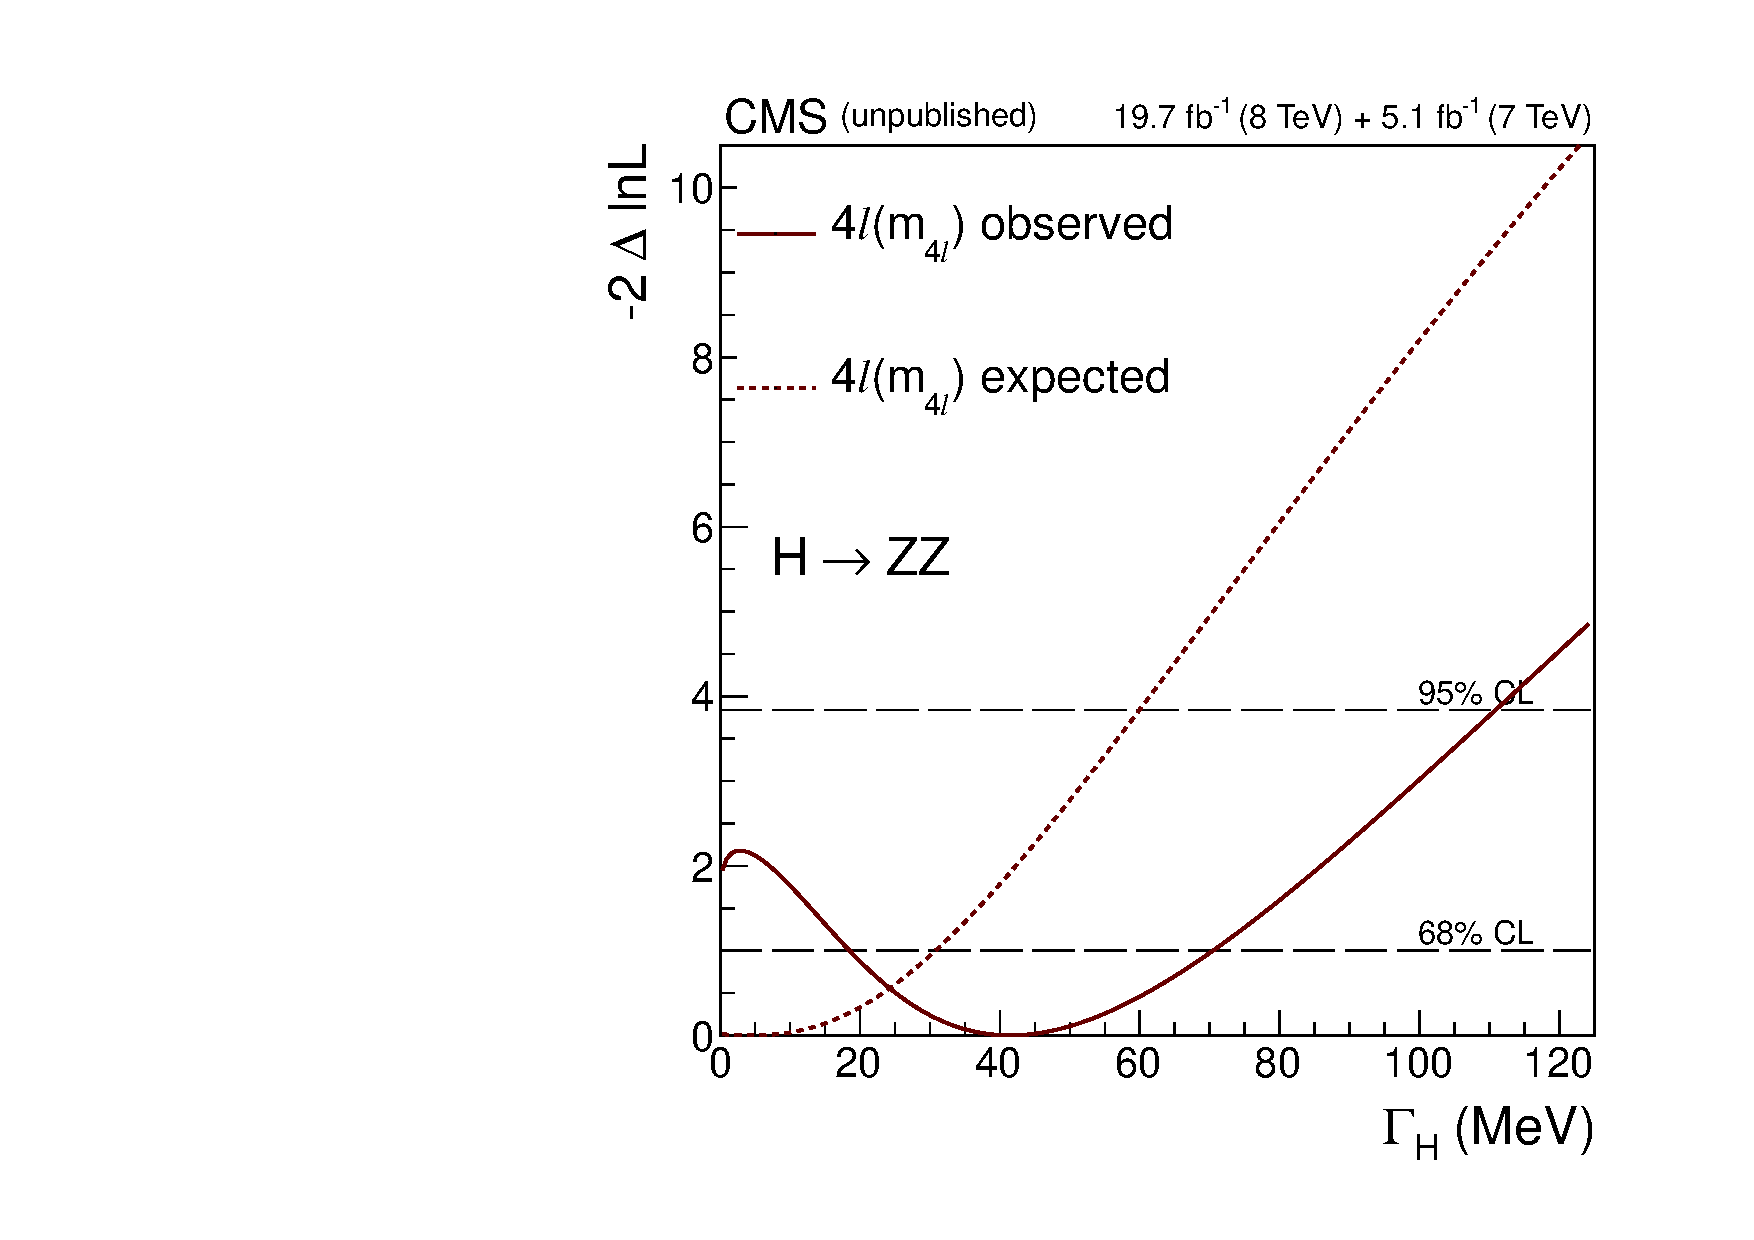
\includegraphics[width=0.45\textwidth]{HZZ_Width/1Dm4lFitPaper_30_04_14_MeV.pdf}
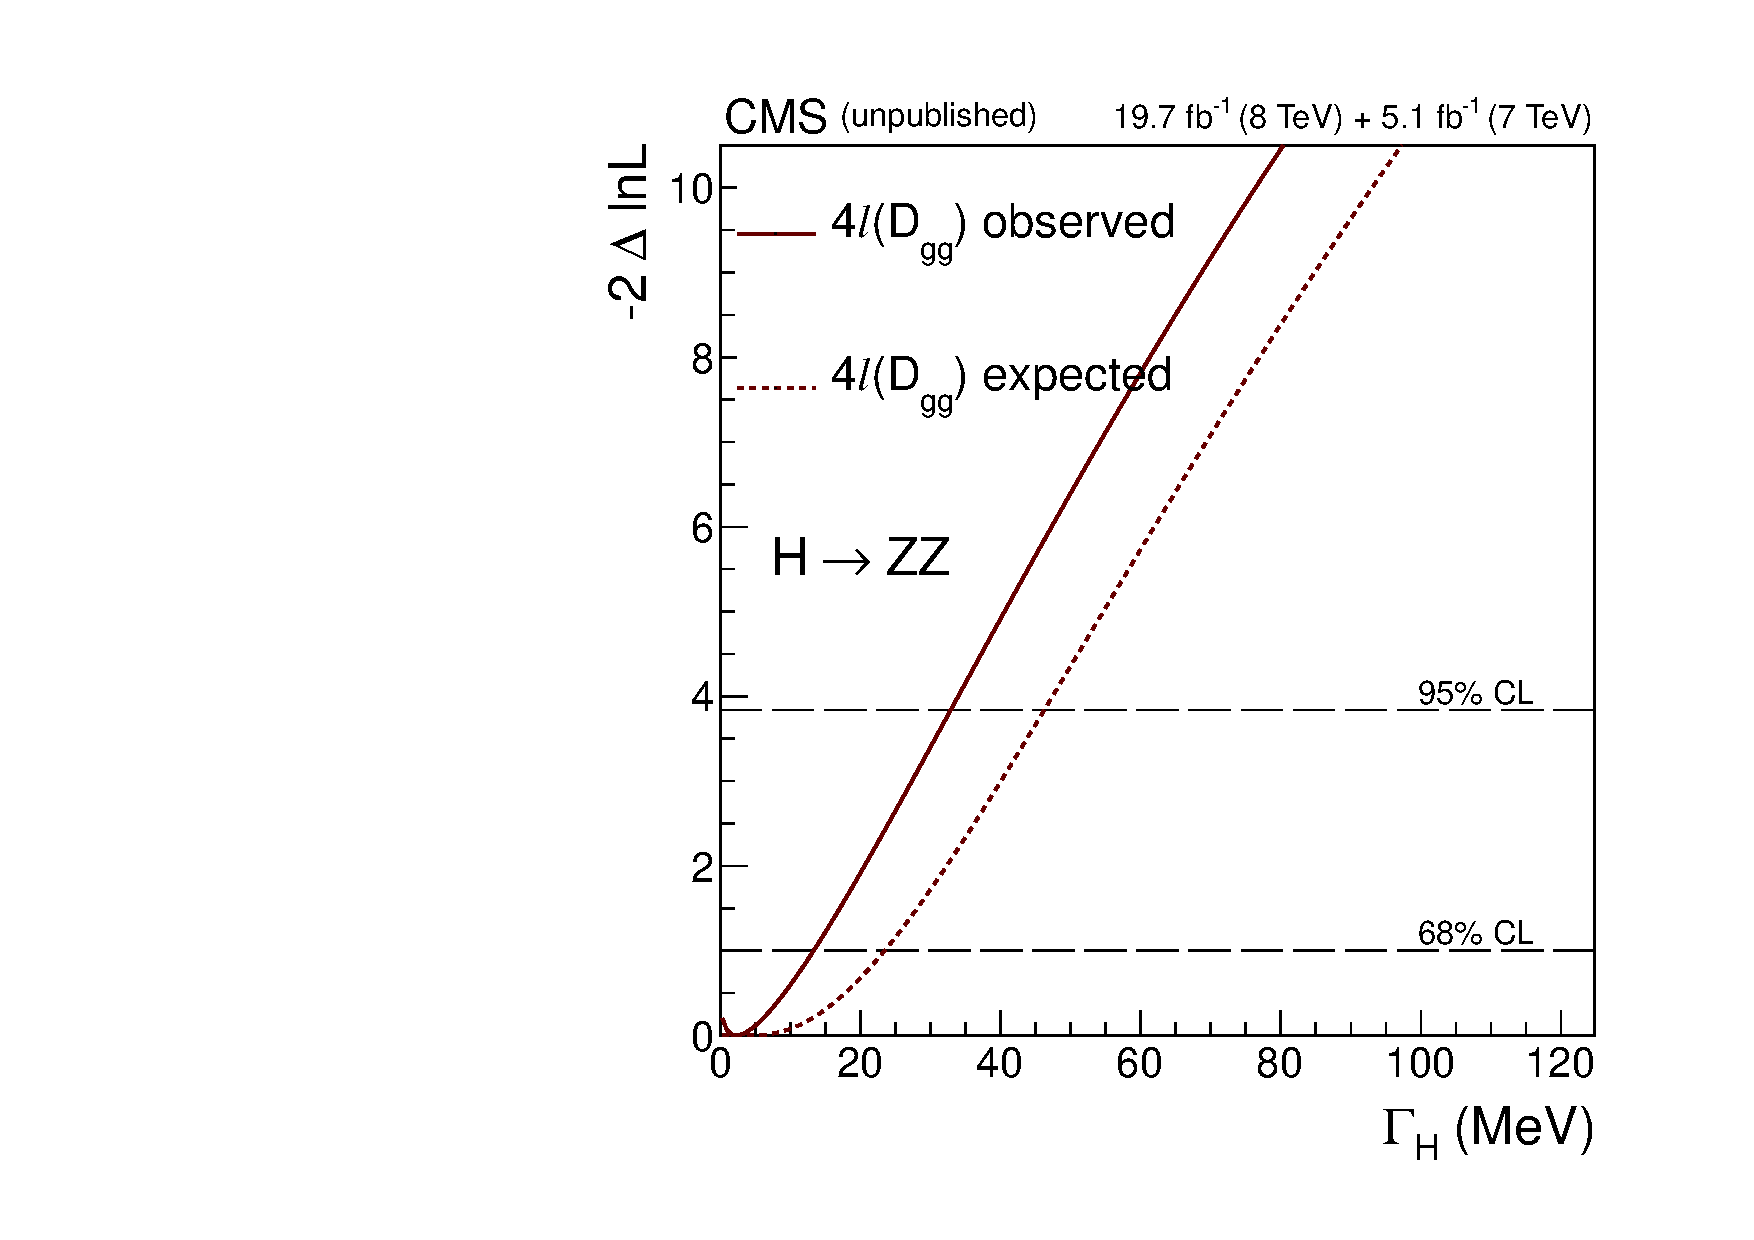
\includegraphics[width=0.45\textwidth]{HZZ_Width/1DDggFitPaper_30_04_14_MeV.pdf}
\end{center}
\end{figure}

The full fit results are shown in figure \ref{fig:finalplot} and summarized in table \ref{tab:Fit_results}.
Combining the $4\ell$ and $2\ell2\nu$ channels a limit is observed (expected) on the total width of $\Gamma_{H} < \unit{22}{\MeV}$
($\unit{33}{\MeV}$) at a 95\% C.L., which is 5.4 (8.0) times the expected value in the SM.
The best fit value and 68\% C.L. interval correspond to $\Gamma_{H} = 1.8^{+7.7}_{-1.8}\unit{}{\MeV}$. The
result of the $4\ell$ analysis alone is an observed (expected) limit of $\Gamma_{H} < \unit{33}{\MeV}$
($\unit{42}{\MeV}$) at a 95\% C.L., which is 8.0 (10.1) times the SM value, and the result of the
analysis combining the $4\ell$ on-shell and $2\ell 2\nu$ off-shell regions is $\Gamma_{H} < \unit{33}{\MeV}$
($\unit{44}{\MeV}$) at a 95\% C.L., which is 8.1 (10.6) times the SM value.
The best fit values and 68\% C.L. intervals are $\Gamma_{H} = 1.9^{+11.7}_{-1.9}\unit{}{\MeV}$ and
$\Gamma_{H} = 1.8^{+12.4}_{-1.8}\unit{}{\MeV}$ for the $4\ell$ analysis and for the analysis combining the $4\ell$
on-shell and $2\ell 2\nu$ off-shell regions, respectively.
\begin{figure}
\centering
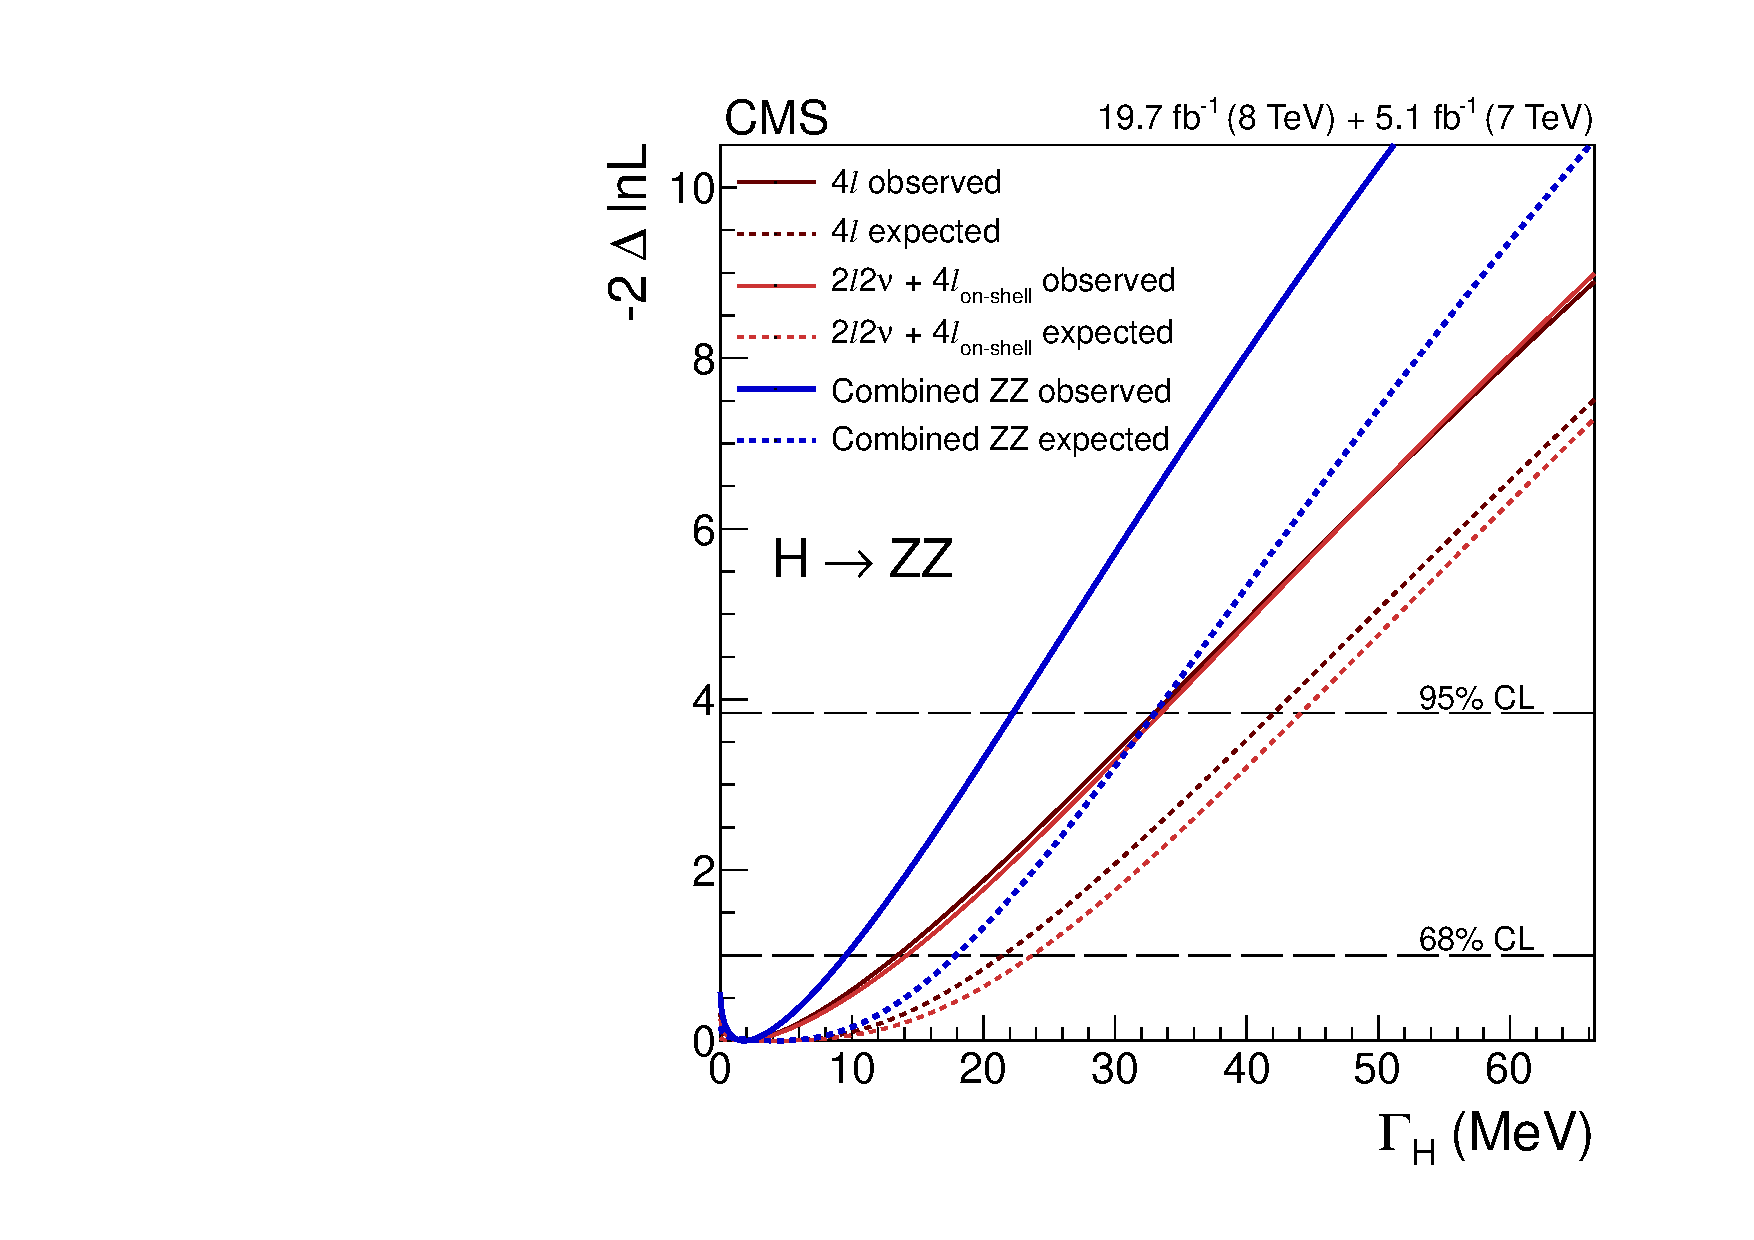
\includegraphics[width=0.75\linewidth]{HZZ_Width/fig5_new.pdf}
\caption[Scan of the negative log-likelihood, $-2 \Delta \ln\mathcal{L}$, as a
function of $\Gamma_{H}$ for the combined fit of the $4\ell$ and
$2\ell 2\nu$ channels (blue thick lines), for the $4\ell$ channel alone in the
off-shell and on-shell regions (dark red lines), and for the $2\ell 2\nu$
channel in the off-shell region and $4\ell$ channel in the on-shell region
(light red lines). The solid lines represent the observed values, the dotted lines
the expected values]{
Scan of the negative log-likelihood, $-2 \Delta \ln\mathcal{L}$, as a
function of $\Gamma_{H}$ for the combined fit of the $4\ell$ and
$2\ell 2\nu$ channels (blue thick lines), for the $4\ell$ channel alone in the
off-shell and on-shell regions (dark red lines), and for the $2\ell 2\nu$
channel in the off-shell region and $4\ell$ channel in the on-shell region
(light red lines). The solid lines represent the observed values, the dotted lines
the expected values \cite{Khachatryan:2014iha}.
}
\label{fig:finalplot}
\end{figure}

\begin{table}
\begin{center}
\caption[Expected and observed 95\% C.L. limits for the $4\ell$ and $2\ell2\nu$ analyses and for the combination. For the observed results, the central fitted values and the 68\% C.L. total uncertainties are also quoted. The Higgs mass is set to the measured value in the $4\ell$ decay channel of $\unit{125.6}{\GeV}$.]{Expected and observed 95\% C.L. limits for the $4\ell$ and $2\ell2\nu$ analyses and for the combination. For the observed results, the central fitted values and the 68\% C.L. total uncertainties are also quoted. The Higgs mass is set to the measured value in the $4\ell$ decay channel of $\unit{125.6}{\GeV}$ \cite{CMS_AN_2014_018,Khachatryan:2014iha}.}
\label{tab:Fit_results}
\begin{tabular}{l | l | c c }
\hline
Analysis & Observed/ & 95\% C.L. limit on &  95\% C.L. limit on \\
               & Expected  &  $\Gamma_{\mathrm{H}}$ ($\MeV$) & $\Gamma_{\mathrm{H}}/\Gamma^{\mathrm{SM}}_{\mathrm{H}}$ \\
\hline \hline
$4\ell \left(m_{4\ell}\right)$ & Expected & 57.7 & 13.9  \\
\hline
& {\bf Observed} & 112.5 & 27.1  \\
\hline\hline
$4\ell \left(\mathcal{D}_{gg}\right)$ & Expected & 44.3 & 10.7 \\
\hline
& {\bf Observed} & 33.0 & 8.0  \\
\hline\hline
$4\ell \left(m_{4\ell}, \mathcal{D}_{gg}\right)$ & Expected & 42 & 10.1 \\
\hline
& {\bf Observed} & 33 & 8.0 \\
\hline\hline
$4\ell_{\mathrm{on-shell}} + 2\ell2\nu$ & Expected & 44 & 10.6 \\
\hline
& {\bf Observed} & 33 & 8.1  \\
\hline\hline
Combined & Expected & 33 & 8.0 \\
\hline
& {\bf Observed} & 22 & 5.4 \\
\hline\hline
\end{tabular}
\end{center}
\end{table}

